\documentclass{patmorin}
\usepackage[UKenglish]{babel}
\usepackage{tabularray}
%
\usepackage{inputenc}
\usepackage[T1]{fontenc}
\usepackage{float,verbatim}
 % Something in here is breaking cleveref
 %\usepackage{lmodern,amsmath,amsthm,amsfonts,amssymb,graphicx,float,microtype,thmtools,underscore,mathtools}
 \usepackage{graphicx,amsmath,amsthm,amsfonts,amssymb,mathtools}
% \usepackage[shortlabels]{enumitem}
% \setlist[itemize]{topsep=0ex,itemsep=0ex,parsep=0ex}
% \setlist[enumerate]{topsep=0ex,itemsep=0ex,parsep=0ex}
% \usepackage[usenames,dvipsnames,svgnames,table]{xcolor}
% \usepackage[dvipsnames]{xcolor}
%%%%
% \usepackage[unicode=true]{hyperref}
% \hypersetup{
% 	colorlinks,
% 	linkcolor={blue!60!black},
% 	citecolor={black},
% 	urlcolor={blue!60!black},
% 	pdftitle={Grid Minors and Products}}
%%%
\usepackage[capitalise, compress, nameinlink, noabbrev]{cleveref}
\crefname{lem}{Lemma}{Lemmas}
\crefname{thm}{Theorem}{Theorems}
\crefname{cor}{Corollary}{Corollaries}
\crefname{prop}{Proposition}{Propositions}
%%%
\newcommand{\defn}[1]{\textcolor{Maroon}{\emph{#1}}}
\newcommand{\mathdefn}[1]{\textcolor{Maroon}{#1}}
%%%%%%%%%%%%%%%%%%%%%%%%%%%%%%%%%%%%%%%%%%
\usepackage[longnamesfirst,numbers,sort&compress]{natbib}
 \makeatletter
 \def\NAT@spacechar{~}
 \makeatother
 \setlength{\bibsep}{0.4ex plus 0.2ex minus 0.2ex}
%%%%%%%%%%
\usepackage{todonotes}
\graphicspath{{figs/}}
\usepackage{paralist}
\newcommand{\boxprod}{\mathbin{\Box}}
\newcommand{\N}{\mathbb{N}}
%%%%
\newcommand{\half}{\ensuremath{\protect\tfrac{1}{2}}}
\DeclarePairedDelimiter{\floor}{\lfloor}{\rfloor}
\DeclarePairedDelimiter{\ceil}{\lceil}{\rceil}
\DeclarePairedDelimiter{\abs}{\lvert}{\rvert}
\DeclarePairedDelimiter{\set}{\{}{\}}
%%%% Commands
\renewcommand{\epsilon}{\varepsilon}
\renewcommand{\emptyset}{\varnothing}
\renewcommand{\ge}{\geqslant}
\renewcommand{\le}{\leqslant}
\renewcommand{\geq}{\geqslant}
\renewcommand{\leq}{\leqslant}
%%%
\DeclareMathOperator{\polylog}{polylog}
\DeclareMathOperator{\wcol}{wcol}
\DeclareMathOperator{\col}{col}
\DeclareMathOperator{\dist}{dist}
\DeclareMathOperator{\tw}{tw}
\DeclareMathOperator{\gm}{gm}
\DeclareMathOperator{\tpw}{tpw}
\DeclareMathOperator{\pw}{pw}
\DeclareMathOperator{\td}{td}
\DeclareMathOperator{\sep}{sep}
\DeclareMathOperator{\stw}{stw}
\DeclareMathOperator{\ltw}{ltw}
\DeclareMathOperator{\rtw}{rtw}
%%
\newcommand{\RR}{\mathbb{R}}
\newcommand{\JJ}{\mathcal{J}}
\newcommand{\PP}{\mathcal{P}}
\newcommand{\BB}{\mathcal{B}}
\newcommand{\FF}{\mathcal{F}}
\newcommand{\GG}{\mathcal{G}}
\newcommand{\HH}{\mathcal{H}}
\newcommand{\LL}{\mathcal{L}}
\newcommand{\NN}{\mathbb{N}}
\newcommand{\OO}{\mathcal{O}}
\newcommand{\WW}{\mathcal{W}}
\newcommand{\scr}[1]{\mathcal{#1}}
\newcommand{\ds}[1]{\mathbb{#1}}
%%%
%\newcommand{\david}[1]{{\color{orange} DRW: #1}}
%\newcommand{\vida}[1]{{\color{DarkGreen} V: #1}}
%\newcommand{\pat}[1]{\textcolor{Maroon}{PM: #1}}
%\newcommand{\worley}[1]{\textcolor{Purple}{DAW: #1}}
%%%
 \renewcommand{\thefootnote}{\fnsymbol{footnote}}
%%%
\theoremstyle{plain}
\newtheorem{thm}{Theorem}
\newtheorem{lem}[thm]{Lemma}
\newtheorem{cor}[thm]{Corollary}
\newtheorem{ques}[thm]{Question}
\newtheorem{prop}[thm]{Proposition}
\newtheorem{obs}[thm]{Observation}
\newtheorem*{claim}{Claim}
\crefname{obs}{Observation}{Observations}
\newtheorem*{lem*}{Lemma}
\theoremstyle{definition}
\newtheorem{conj}[thm]{Conjecture}
\newtheorem*{conj*}{Conjecture}
%%%%%%%%%%%%%%%%%%%%%%%%%%%%%%%%%%%%%%%%%%%%%%
\let\oldsubset\subset
\newcommand{\subsetsim}{\mathrel{\ooalign{\raise0.175ex\hbox{$\oldsubset$}\cr\hidewidth\raise-0.9ex\hbox{\scalebox{0.9}{$\sim$}}\hidewidth\cr}}}
%%%%%%%%%%%%%%%%%%%%%%%%%%%%%%%%%%%%%%%%%%%%%%


\begin{document}
\title{\MakeUppercase{Grid Minors and Products}}

\author{
Vida Dujmovi{\'c}\,\footnotemark[3]\qquad
Pat Morin\,\footnotemark[4]\qquad
David~R.~Wood\,\footnotemark[2]\qquad
David~Worley\footnotemark[5]
}

\maketitle

\begin{abstract}
  Motivated by 
  %recent approximation algorithms for NP-hard problems on planar graphs that make use of bidimensionality and the subquadratic grid minor property \david{it seems strange to say we are motivated by bidimensionality and then never mention bidimensionality in the paper itself. The subquadratic grid minor property is mentioned only once, and then only to say products don't have this property. I think we need to either drop this comment from the abstract, or add some discussion about bidimensionality and the subquadratic grid minor property to the paper. If we add this discussion then we need to be careful that we do not present our results as all negative.} \pat{I'm happy to drop the mention of approximation algorithms since all our results are indeed negative in that context.} \david{done} and by 
  recent developments regarding the product structure of planar graphs, we study relationships between treewidth, grid minors, and graph products.  We show that the Cartesian product of any two connected $n$-vertex graphs contains an $\Omega(\sqrt{n})\times\Omega(\sqrt{n})$ grid minor.  This result is tight: The lexicographic product (which includes the Cartesian product as a subgraph) of a star and any $n$-vertex tree has no $\omega(\sqrt{n})\times\omega(\sqrt{n})$ grid minor.
\end{abstract}

\footnotetext[3]{School of Computer Science and Electrical Engineering, University of Ottawa, Ottawa, Canada (\texttt{vida.dujmovic@uottawa.ca}). Research supported by NSERC.}

\footnotetext[4]{School of Computer Science, Carleton University, Ottawa, Canada (\texttt{morin@scs.carleton.ca}). Research supported by NSERC.}

\footnotetext[2]{School of Mathematics, Monash University, Melbourne, Australia (\texttt{david.wood@monash.edu}). Research supported by the Australian Research Council. }

\footnotetext[5]{School of Computer Science and Electrical Engineering, University of Ottawa, Ottawa, Canada (\texttt{dworl020@uottawa.ca}). Research supported by NSERC.}

%\newpage
%\section{\Large Introduction}

 \renewcommand{\thefootnote}{\arabic{footnote}}

\section{Introduction}
\label{Intro}

% \david{I think the introduction would be better structured as follows:
% \begin{itemize}
%     \item treewidth and why it is important
%     \item grid minor theorem as a fundamental result of \citet{RS-V}: there is a function $f$ such that for every integer $k$ every graph with treewidth at least $f(k)$ contains a $k\times k$ grid minor. 
%     \item best known lower and upper bounds on $f$ in   grid minor theorem
%     \item better upper bounds in  grid minor theorem for specific graph classes, such as planar graphs and graphs excluding a fixed minor
%     \item applications of better upper bounds in  grid minor theorem for specific graph classes, bidimensionality, etc.
%     \item we study grid minor theorem for graph products; introduce cartesian, strong, lexicographic products
%     \item motivation for studying grid minor theorem for graph products: (a) natural question since the grid itself is a product, (b) graph product structure theory 
%     \item note that $\tw(G_1\square G_2)\geq n$ for all $n$-vertex connected graphs $G_1$ and $G_2$, and this bound is exactly tight when both $G_1$ and $G_2$ are paths. (I suspect that 
% $\tw(T_1\square T_2)= n$ for all $n$-vertex trees.) 
% So it make sense for a grid minor theorem for products to be in terms of $n$,
%     \item main result 
%     $$\gm(G_1\cdot G_2) \geq \gm(G_1\boxtimes G_2) \geq \gm(G_1\boxprod G_2) \in \Omega(\sqrt{n})$$ 
%     \item upper bound: for any star $S$ and $n$-vertex tree $T$, 
% $$\gm(S\boxprod T) \leq \gm(S\boxtimes T) \leq \gm(S\cdot T) \in O(\sqrt{n})$$
%     \item consequences of main results 
%     \item comparison with known lower and upper bounds on the treewidth of graph products \citep{HW23,WoodJGT13}
%     \item related results on the Hadwiger number of graph products~\citep{Wood-NYJM11}
% \end{itemize}}

% Recently, \emph{graph product structure theory} has been used to resolve a number of longstanding open problems on planar and related graph classes as well as improve various bounds on these classes \cite{DEJGMM21,DFMS21,DEJWW20,DEHMW22}.  In a nutshell, these results are enabled by showing that every planar graph $G$ is isomorphic to a subgraph of the strong
% product of two very simple graphs, a graph $H$ of bounded treewidth and a path $P$, written as $G\subseteq H\boxtimes P$.  Although $H\boxtimes P$ is a supergraph of the original graph $G$, it often shares or inherits properties of $G$, and its obvious structure makes it easier to work with. An obvious (local) example is that any induced subgraph of $H\boxtimes P$  of diameter $k$ has treewidth $O(k)$. For a more global example, any $n$-vertex subgraph of $H\boxtimes P$ has a balanced separator of size $O(\sqrt{n})$.  The proofs of both of these facts are considerably simpler than the same result for planar graphs.  This motivates the need for a deeper understanding of graph products of simple graphs.  Before describing our results, we first define the two types of graph products that we consider.

% The \defn{Cartesian product} of two graphs $G_1$ and $G_2$, denoted $G_1 \boxprod G_2$, is the graph with vertex set $V(G_1 \boxprod G_2) = V(G_1) \times V(G_2)$ where two distinct vertices $(u_1, v_1)$ and $(u_2, v_2)$ are adjacent iff 
% \begin{compactitem}
%     \item $u_1 = u_2$ and $(v_1, v_2) \in E(G_2)$, or
%     \item $v_1 = v_2$ and $(u_1, u_2) \in E(G_1)$.
% \end{compactitem}

% The \defn{strong product} of two graphs $G_1$ and $G_2$, denoted $G_1 \boxtimes G_2$, is the graph with vertex set $V(G_1) \times V(G_2)$ where two distinct vertices $(u_1, v_1)$ and $(u_2, v_2)$ are adjacent iff 
% \begin{compactitem}
%     \item $u_1 = u_2$ and $(v_1, v_2) \in E(G_2)$, 
%     \item $v_1 = v_2$ and $(u_1, u_2) \in E(G_1)$, or
%     \item $(u_1, u_2) \in E(G_1)$ and $(v_1, v_2) \in E(G_2)$.
% \end{compactitem}

% The Planar Graph Product Structure Theorem discussed above asserts that, for every planar graph $G$, there is a graph $H$ of treewidth at most $8$\footnote{This treewidth bound was improved to 6 by \citet{UWY22}.} and a path $P$ such that $G$ is isomorphic to a subgraph of $H\boxtimes P$ \cite{DJMMUW20}. Essentially, the results mentioned above  are all proven by showing that some graph parameter is bounded for $H\boxtimes P$ when $H$ has bounded treewidth and $P$ is a path.  For monotone graph parameters,\footnote{A graph parameter $f(\cdot)$ is \defn{monotone} if $f(A)\le f(B)$ whenever $A$ is isomorphic to a subgraph of $B$.} this implies that the parameter is bounded for all planar graphs.  These results therefore imply that many important properties of planar graphs are shared by graph products of the form $H\boxtimes P$.


% % to prove that the class of planar graphs has bounded queue number by modelling them as a subgraph of the product of a path and a graph with bounded treewidth.
% % This resolved a longstanding conjecture of Heath and Rosenberg \cite{HLR92} and resulted in increased focus on research in graph product structure theory. Since then, graph product structure theory has been used to solve various open problems across different areas of graph theory such as graph colouring, adjacency labelling, data structures, and now, grid minors. %\cite{DEJGMM21}
% % \worley{Should I cite some examples of papers here or keep citations strictly research related?} \pat{Yes, put a long string of citations here.}


% % This research was also motivated by the hope of applying the subquadratic grid minor (SQGM) framework to graph products. Unfortunately, our results prove this is not possible for the product of general graphs $G_1$ and $G_2$.

% % TODO: Define the subquadratic grid minor property and the state-of-the art in excluded grid minors.

% The \defn{Excluded Grid Theorem for Planar Graphs} asserts that planar graphs have the \defn{linear grid minor property}, i.e., that any planar graph of treewidth at least $k$ contains an $\Omega(k)\times \Omega(k)$ grid minor.  This property has been used to devise efficient polynomial time approximation schemes for many NP-hard problems on planar graphs and related graph families\cite{DHK-Algo09,DFHT-JACM05,DH-Algo04, Eppstein-Algo00, FFLS18}.

% \david{\citet{KK20} is an important reference here. They give an explicit function $f$ such  that every graph with treewidth at least $f(t)k$ has a $k\times k$ grid minor or a $K_t$-minor, and the proof does not use the graph minor structure theorem.}

% General graphs do not have this property; there are graphs of treewidth $k^2\log k$ whose largest grid minor is of size $O(k)\times O(k)$ \cite{RST-JCTB94}.  Currently, the best known \defn{Excluded Grid Theorem} (for general graphs) asserts that any graph of treewidth at least
% $k^{9+\epsilon}$ contains a grid minor of size $\Omega(k)\times\Omega(k)$ \cite{CT21}.  In the current work, we consider the question of whether the linear grid minor property---or something close to it---can be preserved in the product.  In short, the answer is no \david{This sounds very negative, whereas I think our results are actually very positive. We prove tight bounds on the size of grid minors in cartesian products of connected graphs. This is the way to present the results, rather than starting with the question of whether cartesian products have the linear grid minor property (even if this research started by thinking about whether cartesian products have the linear grid minor property).}  We now describe our results in more detail.

% For every positive integer $k$, let $P_k$ be the path on $k$ vertices and let $\boxplus_k:=P_k\boxprod P_k$ denote the $k\times k$ \defn{grid graph}.\footnote{For every positive integer $k$, let $[k]:=\{1,\ldots,k\}$. \pat{Is this notation still used?}}  For a graph $G$, let $\tw(G)$ denote the treewidth\footnote{A \defn{tree-decomposition} of a graph $G$ is a collection $(B_x :x\in V(T))$ of subsets of $V(G)$ (called \defn{bags}) indexed by the vertices of a tree $T$, such that (a) for every edge $uv\in E(G)$, some bag $B_x$ contains both $u$ and $v$, and (b) for every vertex $v\in V(G)$, the set $\{x\in V(T):v\in B_x\}$ induces a non-empty (connected) subtree of $T$. The \defn{width} of $(B_x:x\in V(T))$ is $\max\{|B_x| \colon x\in V(T)\}-1$. 
% %A \defn{path-decomposition} is a tree-decomposition in which the underlying tree is a path, simply denoted by the corresponding sequence of bags $(B_1,\dots,B_n)$. 
% The \defn{treewidth} of a graph $G$, denoted by \defn{$\tw(G)$}, is the minimum width of a tree-decomposition of $G$.
% } of $G$ and let $\gm(G)$ denote the largest integer $k$ such that $G$ contains a $\boxplus_k$ minor.\footnote{A graph $G_1$ is a \defn{minor} of a graph $G_2$ if a graph isomorphic to $G_1$ can be obtained from a subgraph of $G_2$ through a sequence of edge contractions.}

% In this paper, we prove the following results:

% \begin{enumerate}
%    \item  For any two $n$-vertex connected graphs $G_1$ and $G_2$, $\gm(G_1\boxprod G_2) \in \Omega(\sqrt{n})$ (see \cref{lower_bound}).
%    \item There exists two $n$-vertex connected graphs $G_1$ and $G_2$ (a star and a path) such that $\gm(G_1\boxtimes G_2) \in O(\sqrt{n})$ (see \cref{upper_bound}).  
% \david{A star and any $n$-vertex tree has this property; see \cref{StarTreeUpperBound}}

% \end{enumerate}

% Pat is working here...

% % \citet[Theorem~2]{WoodJGT13} shows that the Cartesian product of any two connected $n$-vertex graphs has treewidth at least $n-1$.  It is not difficult to show that, for any two graphs $G_1$ and $G_2$, $\tw(G_1\boxtimes G_2)\le (\tw(G_1)+1)|V(G_2)|-1$. 



% % Thus, for any tree $T$ and any $n$-vertex graph $G$, $\tw(T\boxtimes G)\le 2n-1$.


% % In particular, products of the form $H\boxtimes P$


% % Thus, our second result shows that $(n,1)$-products do not have the linear (or even subquadratic) grid minor property.


% % Say that a graph $G$ is an \defn{$(n,w)$-product} if it is the product of two $n$-vertex connected graphs, each of treewidth at most $w$.  Thus, our first result shows that every $(n,w)$-product contains an $\Omega(\sqrt{n})\times\Omega(\sqrt{n})$ grid minor and the second result shows that bound is asymptotically tight for some $(n,1)$-products.   




% %   Thus, our first result 


% % $T$ and any $n$-vertex connected graph $G$, $\tw(T\boxtimes G) \le (\tw(T)+1)$ $\tw(T\boxprod G)$ and $\tw(T\boxtimes G)$ are both in $\Theta(n)$.\footnote{An upper bound of $O(n)$ comes follows from the fact that $\tw(T\boxtimes G)\le (\tw(T)+1)\cdot |V(G)|-1$.  For the lower bound, \citet[Theorem 2]{WoodJGT13} shows that, for any two connected $n$-vertex graphs $G_1$ and $G_2$, $\tw(G_1\boxprod G_2)\ge n-1$.}
% % when $T_1$ and $T_2$ are $n$-vertex trees \cite{HW}
% % \david{Actually, $\tw(T\boxprod G)\in\Theta(n)$ when $T$ is any $n$-vertex tree and $G$ is any connected $n$-vertex graph.}.  
% Thus, the first result above gives an excluded grid theorem for graph products that is stronger than what is possible for general graphs and much stronger than what can be proven for general graphs. 


% The second result shows that the first result is tight for both the Cartesian and strong product of two trees.  A consequence of the second result is that there exists two trees whose product has treewidth at most $n$ but whose largest grid minor has size $O(\sqrt{n})\times O(\sqrt{n})$.  Thus, even these simple products do not have the linear (or even subquadratic) grid minor property. 

% The remainder of this paper is organized as follows:  In \cref{A} we discuss background material. In \cref{B} we prove the lower bound. In \cref{C} we prove the upper bound. \Cref{D} summarizes and concludes with directions for future work.

% % Unfortunately, our lower bound falls just short of being strong enough to allow the SQGM framework to be directly applied to graph products and the upper bound in the second result shows that this is by necessity.  TODO: Point to future work.

% \worley{Working on a restructured introduction here. }


Treewidth\footnote{A \defn{tree-decomposition} of a graph $G$ is a collection $(B_x :x\in V(T))$ of subsets of $V(G)$ (called \defn{bags}) indexed by the vertices of a tree $T$, such that (a) for every edge $uv\in E(G)$, some bag $B_x$ contains both $u$ and $v$, and (b) for every vertex $v\in V(G)$, the set $\{x\in V(T):v\in B_x\}$ induces a non-empty (connected) subtree of $T$. The \defn{width} of $(B_x:x\in V(T))$ is $\max\{|B_x| \colon x\in V(T)\}-1$. 
%A \defn{path-decomposition} is a tree-decomposition in which the underlying tree is a path, simply denoted by the corresponding sequence of bags $(B_1,\dots,B_n)$. 
    The \defn{treewidth} of a graph $G$, denoted by \defn{$\tw(G)$}, is the minimum width of a tree-decomposition of $G$.} is a ubiquitous parameter in structural graph theory measuring how close a graph is to a tree. It was first introduced as \textit{dimension} by \citet[pp.~37--38]{BB1972} in 1972, then rediscovered by \citet{Halin76} in 1976. The parameter was popularized when it was once again rediscovered by Robertson and Seymour~\cite{ROBERTSON198449} in 1984 and has since been at the forefront of structural graph theory research. Graphs of bounded treewidth are of particular interest due to the wide implications of their tree-like structure. For example, Courcelle's Theorem~\cite{Courcelle90} implies that many NP-Complete problems can be solved in linear time on graphs of bounded treewidth. 

Another key way to study the structure of graphs is through analysis of their minors.\footnote{A graph $G_1$ is a \defn{minor} of a graph $G_2$ if a graph isomorphic to $G_1$ can be obtained from a subgraph of $G_2$ through a sequence of edge contractions.} Finding a highly structured minor of a graph $G$ allows us to use properties of the minor to study $G$ itself. In particular, we are interested in studying the largest $k$ such that the $k\times k$ grid graph $\boxplus_k$ is a minor of $G$, where $\boxplus_k$ is defined to be the Cartesian product of two $k$-vertex paths. Let \defn{$\gm(G)$} be the maximum integer $k$ such that $\boxplus_k$ is a minor of $G$. 
It is folklore that $\tw(\boxplus_k)=k$; see~\citep{HW17} for a proof. 
This, combined with the fact that treewidth is minor-monotone, implies that for every graph $G$, 
\begin{equation}\label{tw_gte_gm}
    \tw(G) \geq \gm(G).
\end{equation}

%A similar structurally impactful parameter is the  Hadwiger Number. The Hadwiger Number of a graph $G$, denoted $h(G)$ is the largest integer $n$ is such that $G$ contains a $K_n$ minor. We refer interested readers to \cite{todo} \worley{Find a survey for this} for a survey on this area, as our work will focus on the aformentioned grid minors. 

%\david{Somewhere near here we need to say that the $k\times k$ grid has treewidth $k$. And since treewidth is minor-monotone, $\tw(G)\geq\gm(G)$ for every graph $G$. This is essential for the narrative, and we use it later.} \worley{Incorporated into previous paragraph}

A foundational result in this area is the \defn{Grid Minor Theorem} (also known as the \defn{Excluded Grid Theorem}) of Robertson and Seymour~\cite{RS-V}, which says there exists a function $f$ such that for every positive integer $k$, $f(k)$ is the minimum integer such that every graph with treewidth at least $f(k)$ contains a $k \times k$ grid minor.  Thus grid graphs are canonical examples of graphs with large treewidth. 

This result had widespread impact on structural graph theory research and led to further investigation into the best possible bounds for the function $f$. \citet{RS-V} proved the existence of $f(k)$, which they, along with Thomas, later showed to be in $2^{O(k^5)}$~\cite{RST-JCTB94}. \citet{DJGT-JCTB99} showed that if $G$ has treewidth $\Omega(k^{4m^2(k+2)})$ where $k$ and $m$ are integers, then $G$ contains either $K_m$ or the $k \times k$ grid as a minor. \citet{LeafSeymour15} improved the upper bound to $f\in 2^{O(k \log k)}$.  
%\david{None of the proofs of the Grid Minor Theorem use the graph minor structure theorem. It doesn't make sense to use the graph minor structure theorem in a proof of the Grid Minor Theorem since the Grid Minor Theorem is used in the proof of graph minor structure theorem. The main point of the result by Kawarabashi and Kobayashi is that for any graph $H$ there exists $c$ such that for all $k$ every $H$-minor-free graph with treewidth at least $ck$ has a $k\times k$ grid minor. So we get a linear bound in the Grid Minor Theorem for graphs in a proper minor-closed class. This was previously proved by Demaine et al.\ using the graph minor structure theorem, but the proof of  Kawarabashi and Kobayashi is self-contained without using the  the graph minor structure theorem. I suggest we don't mention the Kawarabashi and Kobayashi  result here, and instead incorporate it into the  paragraph below where we discuss the linear grid minor property.}\worley{Fixed bounds and reorganized text accordingly. } 
The first polynomial upper bound, stating that $f \in O(k^{98}\log k)$, was found by Chekuri and Chuzhoy~\cite{CC16}. Chuzhoy continued to work towards lowering this exponent, with the current state-of-the-art result by \citet{CT21} showing that $f \in O(k^9\log^{O(1)}k)$. A lower bound of $f\in \Omega(k^2\log k)$ was shown by Robertson~et~al.~\cite{RST-JCTB94}, and \citet{DHK-Algo09} conjectured $f\in \Theta(k^3)$. 

For particular classes of graphs, much stronger Grid Minor Theorems are known. Say a class $\GG$ has the \defn{linear grid minor property} if, for some constant $c$,  every graph in $\mathcal{G}$ with treewidth at least $ck $ contains $\boxplus_k$ as a minor. For example, 
\citet{RST-JCTB94} showed that every planar graph with treewidth at least $6k$ contains $\boxplus_k$ as a minor. Thus the class of planar graphs has the linear grid minor property. More generally, \citet{DemHaj-EuJC07} proved that every proper minor-closed class has the linear grid minor property. The proof used the Graph Minor Structure Theorem, which in turn depends on the Grid Minor Theorem. \citet{KK20} gave an alternative self-contained proof. In particular, they showed that for any graph $H$ there exists $c\leq |V(H)|^{O(|E(H)|)}$ such that 
every $H$-minor-free graph with treewidth at least $ck$ contains $\boxplus_k$ as minor. 
The linear grid minor property has been used to devise efficient polynomial time approximation schemes for many NP-hard problems on planar graphs and related graph families~\cite{DHK-Algo09,DFHT-JACM05,DH-Algo04, Eppstein-Algo00, FFLS18}. Note that the $\Omega(k^2\log k)$ lower bound mentioned above shows that general graphs do not have the linear grid minor property.

 
%For special classes of graphs, much stronger bounds on $f(k)$ have been shown. One such example is the  \defn{Excluded Grid Theorem for Planar Graphs} 
%\david{I don't see any need to name the ``Excluded Grid Theorem for Planar Graphs''. We do not use this name again.} of Robertson et al.\cite{RST-JCTB94}, which asserts that planar graphs have the \defn{linear grid minor property}, i.e., that for any planar graph, $f(k) \in O(k)$, meaning that any graph with treewidth $O(n)$ contains $\boxtimes_n$ as a minor. \david{This is too vague, since $f$ is not defined with respect to a graph. }\worley{Is this better?}.  This property has been used to devise efficient polynomial time approximation schemes for many NP-hard problems on planar graphs and related graph families~\cite{DHK-Algo09,DFHT-JACM05,DH-Algo04, Eppstein-Algo00, FFLS18}. Demaine at al. proved that every minor-closed family of graphs exhibits the linear grid minor property \cite{DemHaj-EuJC07}. This was also proven by Kawarabashi and Kobayashi in \cite{KK20}, this proof was of particular interest as the result is self-contained, with no reliance on the graph minor structure theorem. The $\Omega(k^2\log k)$ lower bound mentioned above shows that general graphs do not have the linear grid minor property: there are graphs of treewidth $k^2\log k$ whose largest grid minor is of size $O(k)\times O(k)$~\cite{RST-JCTB94}. %The best results for general graph products are found through applications of the best known grid minor theorem from \cite{CT21}, combined with the bounds on treewidth of graph products discovered by Wood\cite{HW23, WoodJGT13}. In the current work, we look into improve these bounds for graph products by analyzing the structure of said products directly.

%\worley{This paragraph needs some work.}
%The Grid Minor Theorem has since been used to improve upper and lower bounds for a multitude of different properties on specific graph classes, one example is [\worley{TODO}]. The theorem has seen further applications and revisions across graph theory. 
%\pat{I would leave out the next reference.  It doesn't have any bearing on $f(k)$.}Dujmovic et al. rephrase the Grid Minor Theorem in terms of product structure and use this to qualitatively improve the theorem \cite{DHHJLMMRW23}, they then show this can be used to improve the upper bound for the weak colouring number of graphs excluding a fixed minor. \worley{More applications?}

In this paper, we study grid minors in graph products\footnote{See \citep{EH20,HW23,WoodJGT13,EFM22,KOY14,CK06} for related work on the treewidth of graph products, and see \citep{BM98,Wood-NYJM11} for related work on complete graph minors in graph products.}.  This is motivated both by the fact that the grid graph itself is the Cartesian product of two paths, and also by recent developments in Graph Product Structure Theory. This area of research studies complex graph classes by modelling them as a product of simpler graphs and investigating the properties of these highly structured supergraphs. 
Before discussing Graph Product Structure Theory further, we first define the three types of graph products that we consider, each illustrated in \cref{Products}. Let $G_1$ and $G_2$ be graphs. 
The \defn{Cartesian product} of  $G_1$ and $G_2$, denoted $G_1 \boxprod G_2$, is the graph with vertex set $V(G_1) \times V(G_2)$ where two distinct vertices $(u_1, v_1)$ and $(u_2, v_2)$ are adjacent iff 
\begin{compactitem}
    \item $u_1 = u_2$ and $v_1v_2 \in E(G_2)$, or
    \item $v_1 = v_2$ and $u_1u_2 \in E(G_1)$.
\end{compactitem}
The \defn{strong product} of  $G_1$ and $G_2$, denoted $G_1 \boxtimes G_2$, is the graph with vertex set $V(G_1) \times V(G_2)$ where two distinct vertices $(u_1, v_1)$ and $(u_2, v_2)$ are adjacent iff 
\begin{compactitem}
    \item $u_1 = u_2$ and $v_1v_2 \in E(G_2)$, 
    \item $v_1 = v_2$ and $u_1u_2 \in E(G_1)$, or
    \item $u_1u_2 \in E(G_1)$ and $v_1v_2 \in E(G_2)$.
\end{compactitem}
The \defn{lexicographic product} of  $G_1$ and $G_2$, denoted $G_1 \cdot G_2$, is the graph with vertex set $V(G_1) \times V(G_2)$ where two distinct vertices $(u_1, v_1)$ and $(u_2, v_2)$ are adjacent iff
\begin{compactitem}
    \item $u_1v_1 \in E(G_1)$, or
    \item $u_1 = u_2$ and $v_1v_2 \in E(G_2)$.
\end{compactitem}
It follows from the above definitions that 
$$G_1\boxprod G_2 \subseteq G_1\boxtimes G_2 \subseteq G_1 \cdot G_2.$$

% \begin{figure}[ht]
% \begin{center}
%   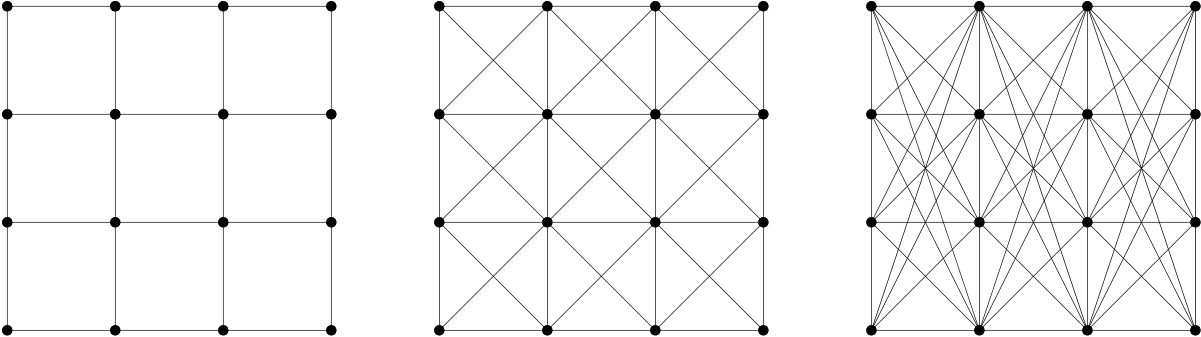
\includegraphics[scale=0.7]{figs/pathProducts-3.ipe.png}
% \end{center}
% \caption{From left to right: $P_4\boxprod P_4$, $P_4\boxtimes P_4$, and $P_4\cdot P_4$ .}
% \label{Products}
% \end{figure}

\begin{figure}[ht]
% \begin{center}
\begin{tblr}{colspec={Q[c]Q[c]Q[c]Q[c]Q[c]Q[c]},rowspec={Q[t]Q[b]}}
 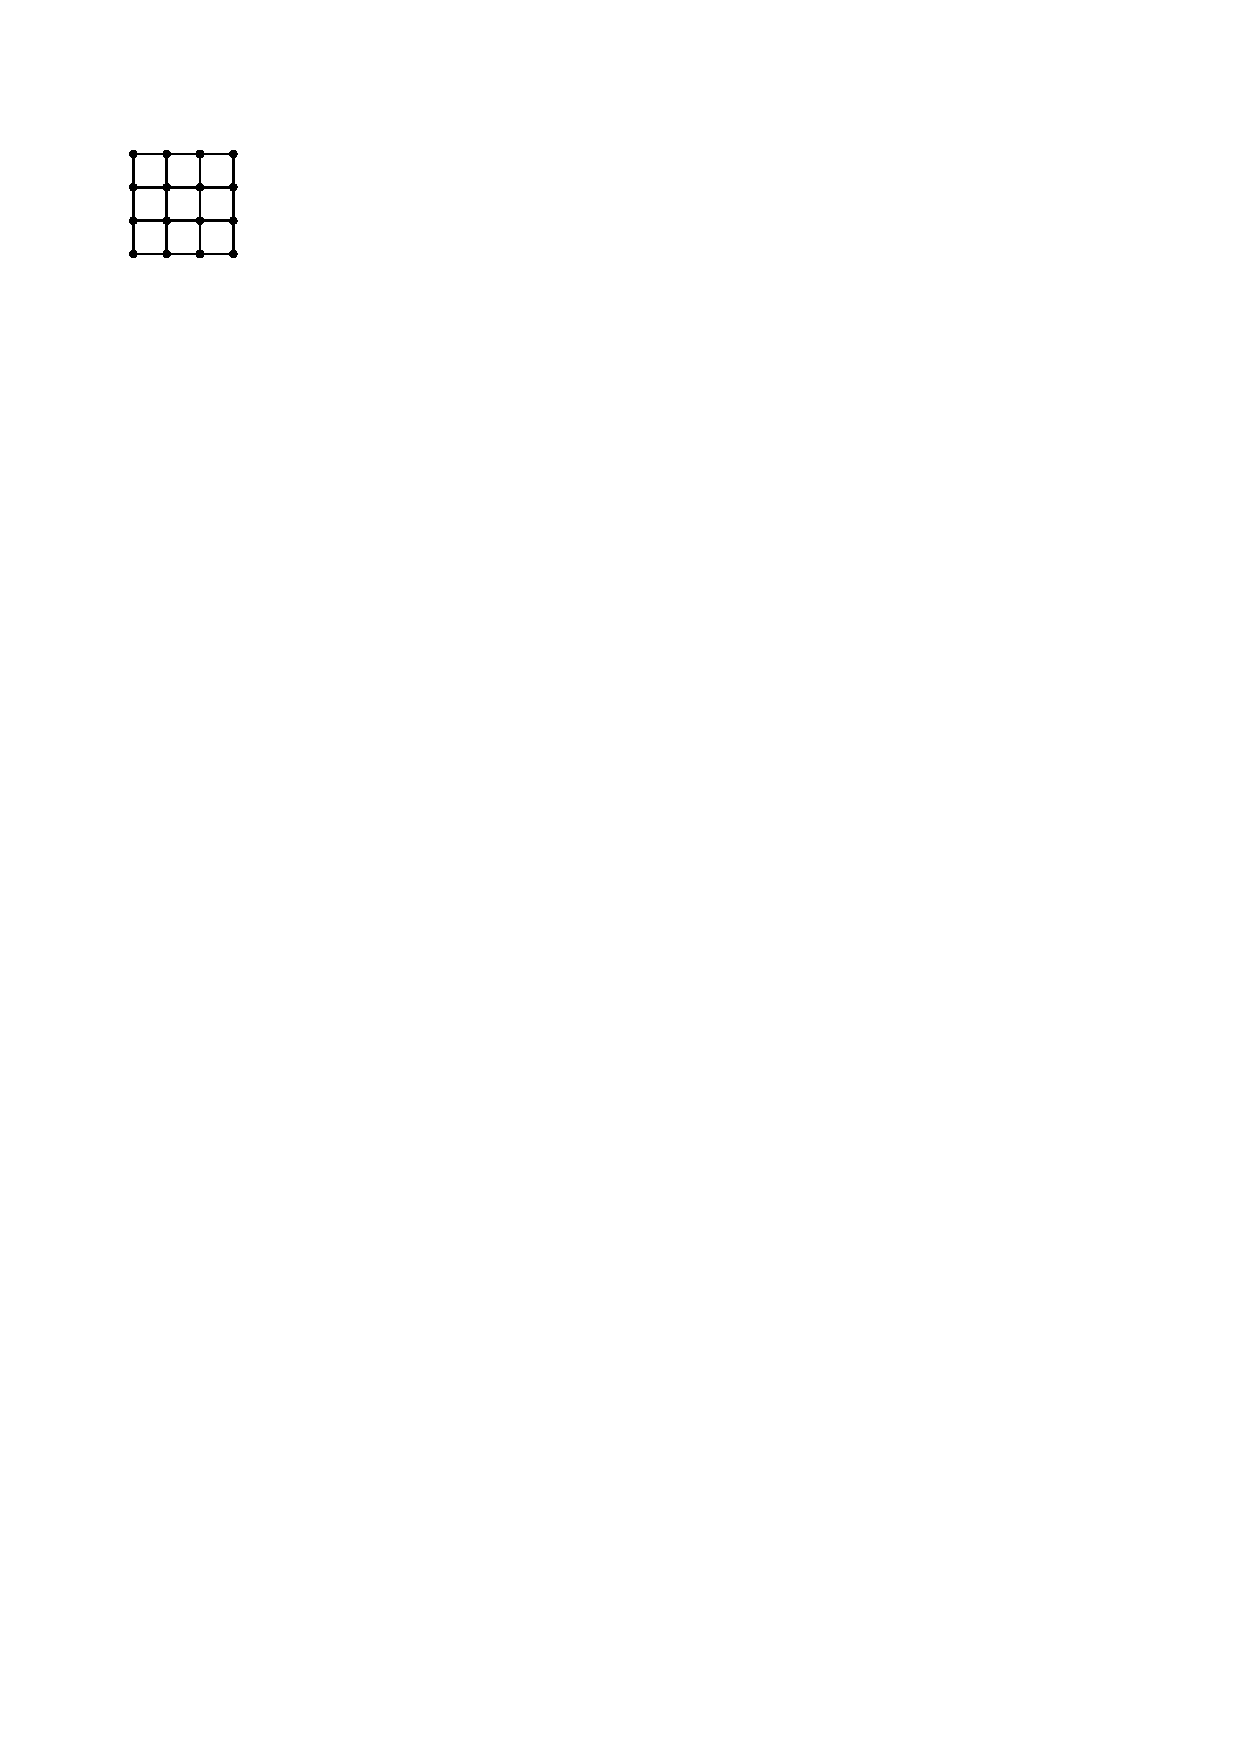
\includegraphics[page=1]{figs/P_4xP_4} &
 \includegraphics[page=2]{figs/P_4xP_4} &
 \includegraphics[page=3]{figs/P_4xP_4} &
 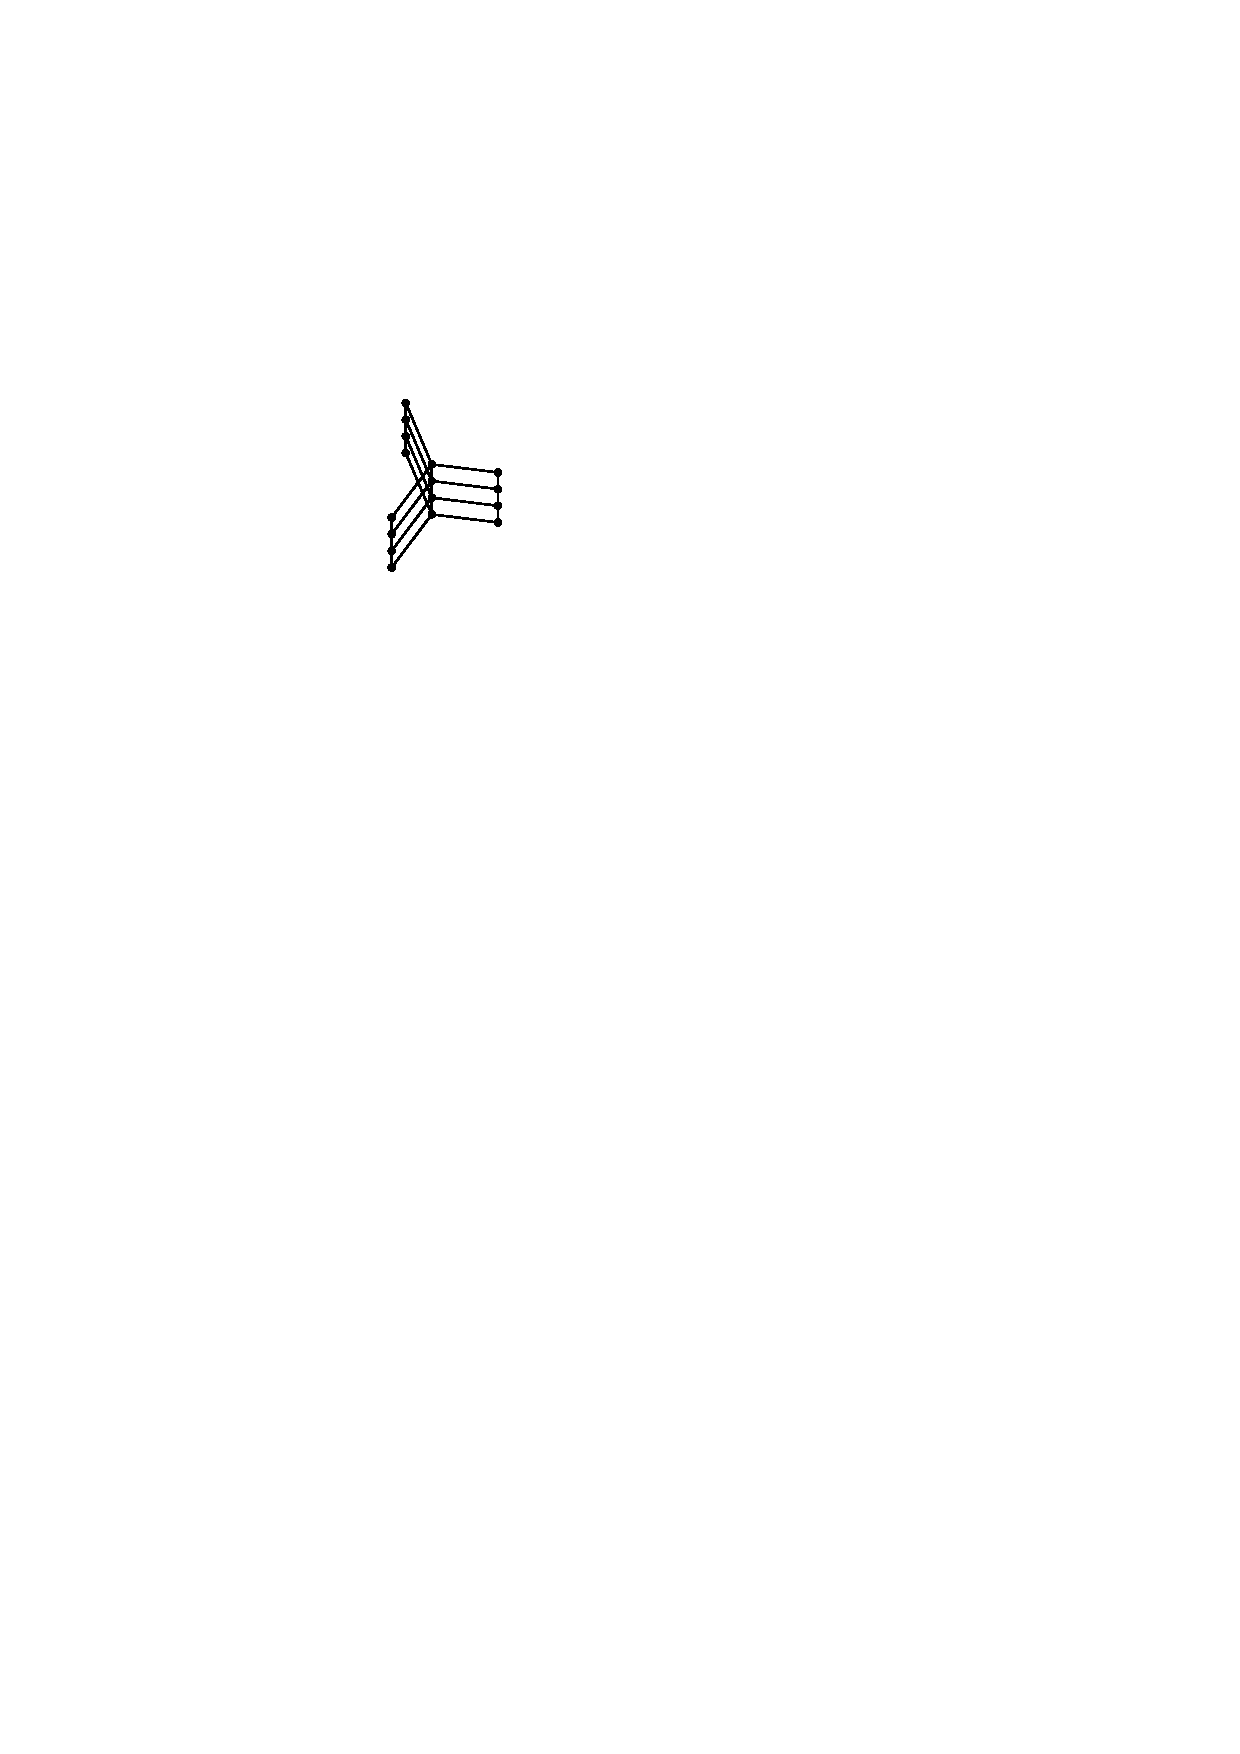
\includegraphics[page=1]{figs/S_3xP_4} &
 \includegraphics[page=2]{figs/S_3xP_4} &
 \includegraphics[page=3]{figs/S_3xP_4} \\
 $P_4\boxprod P_4$ & $P_4\boxtimes P_4$ & $P_4\cdot P_4$ &
 $S_3\boxprod P_4$ & $S_3\boxtimes P_4$ & $S_3\cdot P_4$ 
\end{tblr}
% \end{center}
\caption{The products of two paths and of a star and a path.}
\label{Products}
\end{figure}


%\david{Rotate the third figure 90 degrees, so that vertices correspond to cartesian coordinates.}\worley{fixed}

%\david{The following paragraph should start with a statement of the Planar Graph Product Structure Theorem. This will avoid repetition, and the remainder of the paragraph will make more sense. I suggest we briefly mention generalisations of the Planar Graph Product Structure Theorem for graphs embedded on any surface~\citep{DJMMUW20,DHHW22}, graphs excluding an apex minor~\citep{DJMMUW20,ISW,DHHJLMMRW}, graphs excluding any fixed minor~\citep{DJMMUW20,DEMWW22}, and various non-minor-closed classes~\citep{DMW23,HW21b,DHSW,BDHK22}. Also say that these results have been the key to solving several long-standing open problems  about queue layouts~\citep{DJMMUW20}, nonrepetitive colourings~\citep{DEJWW20}, centred colourings~\citep{DFMS21,DHHJLMMRW}, adjacency labelling~\cite{EJM23,DEJGMM21}, twin-width~\cite{BKW,KPS23,JP22}, vertex ranking~\citep{BDJM}, and box dimension~\citep{DGLTU22}. } \worley{Incorporated these results and updated the next couple paragraphs accordingly.}

The starting point for recent developments in Graph Product Structure Theory is the \defn{Planar Graph Product Structure Theorem} of \citet{DJMMUW20}, which states that every planar graph $G$ is isomorphic to a subgraph of the strong
product of two very simple graphs, a graph $H$ of treewidth\footnote{This treewidth bound was improved to 6 by~\citet{UWY22}.} at most 8 and a path $P$, written as $G\subsetsim H\boxtimes P$.  Although $H\boxtimes P$ is a supergraph of the original graph $G$, it often shares or inherits properties of $G$, and its rigid structure makes it easier to work with. For example, any induced subgraph of $H\boxtimes P$  of diameter $k$ has treewidth $O(k)$. For a more global example, any $n$-vertex subgraph of $H\boxtimes P$ has a balanced separator of size $O(\sqrt{n})$ (see \cite[Lemma~6]{DJMMUW20} and \cite[Lemma~10]{DMW17}).  The proofs of both of these facts are considerably simpler than the same result for planar graphs. 

Product structure theorems have also been developed for other classes of graphs such as surface embeddable graphs~\citep{DJMMUW20,DHHW22}, graphs excluding an apex minor~\citep{DJMMUW20,ISW,DHHJLMMRW}, graphs excluding any fixed minor~\citep{DJMMUW20,DEMWW22}, and various non-minor-closed classes~\citep{DMW23,HW21b,DHSW,BDHK22}. These product structure theorems have been key in resolving many long-standing open problems on queue layouts~\citep{DJMMUW20}, non-repetitive colourings~\citep{DEJWW20}, centred colourings~\citep{DFMS21,DHHJLMMRW}, adjacency labelling~\cite{EJM23,DEJGMM21}, twin-width~\cite{BKW,KPS23-2,JP22}, vertex ranking~\citep{BDJM}, and box dimension~\citep{DGLTU22}. This wide range of applications motivates the need for a deeper understanding of structural properties of graph products. 

%Essentially, the results mentioned above are all proven by showing that some graph parameter is bounded for $H\boxtimes P$ when $H$ has bounded treewidth and $P$ is a path.  For monotone graph parameters,\footnote{A graph parameter $f(\cdot)$ is \defn{monotone} if $f(A)\le f(B)$ whenever $A$ is isomorphic to a subgraph of $B$.} this implies that the parameter is bounded for these graph classes.  These results therefore imply that many important properties of planar graphs are shared by graph products of the form $H\boxtimes P$. \david{I don't understand the reasoning here. What    `important properties of planar graphs' are we refering to? is this paragraph needed? I would delete it.}


\subsection{Our Results}

It is known\footnote{Let $G_1$ and $G_2$ be connected graphs each with at least $n$ vertices. 
For $i\in\{1,2\}$, let $v_i$ be a leaf of a spanning tree of $G_i$, and let $G'_i:=G_i-v_i$, which is connected. For each $x\in V(G'_1)$, let $B_x$ be the subgraph of $G_1\boxprod G_2$ induced by $\{x\}\times V(G'_2)$. 
For each $y\in V(G'_2)$, let $B_y$ be the subgraph of $G_1\boxprod G_2$ induced by $V(G'_1)\times \{y\}$. 
Let $B_1$ be the subgraph of $G_1\boxprod G_2$ induced by $\{v_1\}\times V(G_2)$. 
Let $B_2$ be the subgraph of $G_1\boxprod G_2$ induced by $V(G'_1)\times \{v_2\}$. 
Let $\mathcal{B}:=\{ B_x\cup B_y: x\in V(G'_1),y\in V(G'_2)\}\cup\{B_1,B_2\}$. Then it is easily seen that $\mathcal{B}$ is a bramble in $G_1\boxprod G_2$ of order at least $n+1$. By the Treewidth Duality Theorem~\citep{ST93}, $\tw(G_1\boxprod G_2)\geq n$. This result was extended by \citet{WoodJGT13} who showed that 
for all $k$-connected graphs $G$ and $H$ each with at least $n$ vertices, $\tw(G\boxprod H) \geq k(n-2k+2)-1$. } that for all $n$-vertex connected graphs $G_1$ and $G_2$, 
\begin{equation}
    \label{LowerBoundProduct}
    \tw(G_1 \boxprod G_2) \ge n.
\end{equation}
It thus makes sense for a grid minor theorem for graph products to be in terms of $n$. 
We show that this is in fact the case
by proving the following results:


\begin{enumerate}
   \item  For any two $n$-vertex connected graphs $G_1$ and $G_2$, 
   $$\gm(G_1\cdot G_2) \geq \gm(G_1\boxtimes G_2) \geq \gm(G_1\boxprod G_2) \in \Omega(\sqrt{n})\;\;\text{(see \cref{lower_bound})}.$$
      
   \item There exists two $n$-vertex connected graphs $G_1$ and $G_2$ (a star and any tree) such that   $$\gm(G_1\boxprod G_2) \leq \gm(G_1\boxtimes G_2) \leq \gm(G_1\cdot G_2) \in O(\sqrt{n}) \;\; \text{(see \cref{StarTreeUpperBound})}.$$
   
\end{enumerate}

The previous best bound for the product of two $n$-vertex connected graphs comes from combining \eqref{LowerBoundProduct} with the state-of-the-art Grid Minor Theorem  of Chuzhoy and Tan~\cite{CT21}, giving $\gm(G_1 \boxprod G_2) \in \Omega(n^{1/9}/\polylog(n))$. The first result above gives an excluded grid theorem for graph products that is stronger than what is possible for general graphs and much stronger than what can be proven for general graphs. 


The second result shows that the first result is tight for the Cartesian, strong, and lexicographic product of two trees. %\david{this sentence is strange, since the second result also shows that the first result is tight for the lexicographic product of two trees. I would delete this sentence.}.  
A consequence of the second result and \eqref{LowerBoundProduct} is that there exists two trees whose Cartesian product has treewidth at least $n$ but whose largest grid minor has size $O(\sqrt{n})\times O(\sqrt{n})$. Thus, even these simple products do not have the linear (or even subquadratic) grid minor property. 

The remainder of this paper is organized as follows:  In \cref{A} we discuss background material. In \cref{B} we prove the above lower bound. In \cref{C} we prove the above upper bound. \cref{D} proves some exact bounds for the grid minor number of the products of stars and trees. Finally, \cref{E} concludes with directions for future work.

\section{Preliminaries}\label{A}

For any standard graph-theoretic terminology and notation not defined here, we use the same conventions used in the textbook by~\citet{D10}. In this paper, every graph $G$ is undirected and simple with vertex set $V(G)$ and edge set $E(G)$. The \defn{order} of $G$ is denoted $|G|:=|V(G)|$.  For two graphs $G_1$ and $G_2$ we use the notation $G_1\preceq G_2$ to indicate that $G_1$ is a minor of $G_2$.  We make use of the fact that the $\preceq$ relation is transitive. The following observation follows immediately from definitions.

\begin{obs}\label{minor_product}
  Let $G_1$, $G_2$, and $H$ be graphs.  If $G_1\preceq G_2$, then $G_1\boxprod H\preceq G_2\boxprod H$.
\end{obs}

A \defn{model} of a graph $H$ in a graph $G$ is a set $\mathcal{M}:=\{B_x\subseteq V(G): x\in V(H)\}$ of subsets of $V(G)$, called \defn{branch sets}, indexed by the vertices of $H$ and such that:
\begin{compactenum}[(i)]
  \item for each distinct pair $x,y\in V(H)$, $B_x\cap B_y=\emptyset$;
  \item for each $x\in V(H)$, $G[B_x]$ is connected and
  \item for each $xy\in E(H)$ there exists an edge $vw\in E(G)$ with $v\in B_x$ and $w\in B_y$.
\end{compactenum}
It follows from definitions that $H\preceq G$ if and only if there exists a model of $H$ in $G$.

For each $n\in \N$, let $S_n$ denote the \defn{$n$-star}; the rooted tree with $n$ leaves, each of which is adjacent to the root.  For each $\ell,p\in\N$, let $S_{\ell,p}$ denote the star with $\ell$ leaves whose edges have been subdivided $p-1$ times.  More formally, $V(S_{\ell,p}):=\{v_0\}\cup\{v_{i,j}:(i,j)\in[\ell]\times[p]\}$ and $E(S_{\ell,p}):=\{v_0v_{i,1}:i\in[\ell]\}\cup \{v_{i,j}v_{i,j+1}:(i,j)\in[\ell]\times[p-1]\}$.  We call $S_{\ell,p}$ a \defn{subdivided star}.  Subdivided stars generalize both stars and paths: The $n$-vertex path $P_n$ is isomorphic to $S_{1,n-1}$ and the $n$-leaf star $S_n$ is isomorphic to $S_{n,1}$. 

\begin{lem}\label{anything_times_star}
  For any positive integer $n$ and any $n$-vertex connected graph $G$, $K_{n} \preceq G\boxprod S_n$.
\end{lem}

Note that this lemma is implied by \citep[Lemma~5.1]{Wood-NYJM11}; we include the proof here for the sake of completeness.
\begin{proof}
  Let $y_0$ denote the root of $S_n$, let $y_1,\ldots,y_n$ denote the leaves of $S_n$.  Let $V(K_{n})=[n]$ and let $v_1,\ldots,v_n$ denote the vertices of $G$.  
  We now construct a model $\mathcal{M}:=\{B_x:x\in V(K_n)\}$ of $K_n$ in $G\boxprod S_n$.  For each $i\in V(K_n)$, define the branch set
  \[
     B_i:=\{(v,y_i):v\in V(G)\} \cup \{ (v_{i},y_0) \} \enspace .
  \]
  We now show that $\mathcal{M}$ is a model of $K_n$ in $G\boxprod S_n$.
  The induced graph $(G\boxprod S_n)[B_i]$ is connected because $(G\boxprod S_n)[\{(v,y_i):v\in V(G)\}]$ 
  is isomorphic to $G$ and $(v_{i},y_0)$ is adjacent to $(v_{i},y_i)$.
  For any $1\le i< j\le n$, $B_i$ and $B_j$ are disjoint because $y_i\neq y_j$ and $v_i\neq v_j$.  Furthermore, the vertex $(v_{i},y_0)\in B_i$ is adjacent to $(v_i,y_j)\in B_j$.  Therefore, there is an edge in $G\boxprod S_n$ with one endpoint in $B_i$ and one endpoint of $B_j$ for each $1\le i < j\le n$.
\end{proof}

Note that, for any tree $T$ with $n$ leaves and at least one non-leaf vertex, $S_n\preceq T$.  In this case, \cref{anything_times_star,minor_product} imply that $K_n\preceq G\boxprod T$.

\section{The Lower Bound}\label{B}

% Our lower bound, which shows that, for any two $n$-vertex connected graphs $G_1$ and $G_2$, $\gm(G_1\boxprod G_2)\in\Omega(\sqrt{n})$ is obtained as follows:  We first show that each of $G_1$ and $G_2$ contains a `large' subdivided star.  Then we show that the product of any two `large' subdivided stars $S_{\ell_1, p_1}$ and $S_{\ell_2, p_2}$ contains a large grid-minor.  The quotes on `large' here are due to the fact that we measure the size of a subdivided star in a non-standard way, as in the following lemma.

\subsection{Connected Graphs Contain Large Subdivided Stars}

% We begin with a lemma which shows that every connected $n$-vertex graph contains a model of an $\Omega(n/\log n)$-vertex subdivided star.


% \textbf{Old Lemma and Proof}

% \begin{lem}\label{subdivided_star_minor}
% For every tree $T$ with $n\ge 2$ vertices, there exists integers $\ell,p$ with $\ell p\geq \frac{n-1}{2(\log (n-1)+1)^2}$, a subtree $R$ of $T$ and disjoint paths $P_1,\dots,P_\ell$ in $T-V(R)$, such that for each $i\in\{1,\dots,\ell\}$, one endpoint of $P_i$ is adjacent to some vertex in $R$, and $|V(P_i)|=p$.
% \end{lem}

% \begin{proof}
%   We make use of the \emph{heavy path decomposition} introduced by \citet{ST83} in the context of data structures.  Consider a tree $T$ rooted at a vertex $x$. For each vertex $v$, say a child $w$ of $v$ is \defn{heavy} if the subtree rooted at $w$ has at least as many vertices as each of the subtrees rooted at the other children of $v$. For each vertex $v_1$ of $T$, say a path $(v_1,\dots,v_k)$ in $T$ is \defn{heavy} if $v_{i+1}$ is a heavy child of $v_i$ for each $i\in\{1,\dots,k-1\}$, and $v_k$ is a leaf.

%   Let $\PP=\{P_1,\dots,P_m\}$ be the set of paths obtained from the following algorithm:

% initialise $i:=0$ and $P_0:=\{x\}$ \\
% while $V(T)\neq V(P_0\cup\dots\cup P_i)$ do\\
%  \hspace*{4mm}     increment $i$\\
% \hspace*{4mm} let $T_{i+1}$ be a component subtree of $T-V(P_1\cup\dots\cup P_i)$\\
% \hspace*{4mm} let $P_{i+1}$ be a heavy path in $T_{i+1}$ starting at the root of $T_{i+1}$\\
% end-while

%   Define the \defn{subtree rank} of each $P_i\in\mathcal{P}$ as $\floor{\log_2 |V(T_i)|}$ and define the \defn{length rank} of $P_i$ as  $\floor{\log_2|V(P_i)|}$.  For a path $P_i$, $i\ge 2$, the \defn{parent path} of $P_i$ is the unique path $P_j\in\{P_{1},\ldots,P_{i-1}\}$ that contains the $T$-parent $p$ of the root of $T_i$ (which is the first vertex of $P_i$).  Observe that $p$ has at least two children that root subtrees of size at least $2^r$, where $r$ is the subtree rank of $P_i$. One of these children is the first vertex of $P_i$ and the other is the vertex follows $p$ in $P_j$.  Therefore the subtree rank of $P_j$ is at least $\floor{\log_2 2^{r+1}}=r+1$.  From this, it follows that if two paths in $\PP$ that begin at $x_1,x_2\in V(T)$ have the same subtree rank, then neither  $x_1$ nor $x_2$ is an ancestor of the other.

%   The paths in $\PP$ partition $V(T)\setminus\{x\}$ and each has a subtree rank in the set $\{0,\ldots,\floor{\log_2 (n-1)}\}$.  It follows that, for some $r\in\{0,\ldots,\log_2 (n-1)\}$, the paths in $\PP$ of subtree rank $r$ contain a total of at least $(n-1)/(\floor{\log_2 (n-1)}+1)$ vertices.  By the same reasoning, it follows that for some $s\in\{0,\ldots,\floor{\log_2 (n-1)}\}$, there is a subset $\PP'\subseteq\PP$ that contains a total of at least $(n-1)/(\floor{\log_2 n}+1)^2$ vertices and such that each path in $\PP'$ has subtree rank $r$ and length rank $s$.  Each path in $\PP'$ has length less than $2^{s+1}$, so the number of paths in $\PP'$ is $\ell > (n-1)/2^{s+1}(\floor{\log_2 (n-1)}+1)^2$.  Each path in $\PP'$ has a prefix containing exactly $p:=2^s$ vertices.  Therefore, $p\ell > (n-1)/2(\floor{\log_2 (n-1)}+1)^2$.  Since the paths in $\PP'$ all have the same rank, the component $R$ of $T-\{V(P):P\in\PP'\}$ that contains the root, $x$, of $T$ is adjacent to one endpoint of each path in $\PP'$.
% \end{proof}

We first state some terminology that will be relevant in the following results. The \defn{length} of a path $v_0,\ldots,v_r$ is the number, $r$, of edges in the path. The \defn{depth} of a vertex $v$ in a rooted tree $T$ is the length of the path, in $T$, from $v$ to the root of $T$. A path $P$ in a rooted tree $T$ is \defn{vertical} if, for each $i\in\N$, $V(P)$ contains at most one vertex of depth $i$. The vertex of minimum depth in a vertical path is its \defn{upper endpoint}, and the vertex of maximum depth in a vertical path is its \defn{lower endpoint}. A vertex $v$ is a \defn{$T$-ancestor} of a vertex $w$ if the vertical path from $w$ to the root of $T$ contains $v$.  Two vertices of $T$ are \defn{unrelated} if neither is a $T$-ancestor of the other, otherwise they are \defn{related}.  A pair of paths $P_1$ and $P_2$ in $T$ is \defn{completely unrelated} if $v$ and $w$ are unrelated, for each $v\in V(P_1)$ and each $w\in V(P_2)$.  We say that $P_1$ and $P_2$ are \defn{completely related} if $v$ and $w$ are related, for each $v\in V(P_1)$ and each $w\in V(P_2)$. The \defn{height} $h_T(v)$ of a vertex $v$ in $T$ is the maximum order of a vertical path in $T$ whose upper endpoint is $v$.  For each $i\in\N$, let $\mathdefn{H_i(T)}:=\{v\in V(T):h_T(v)=i\}$ and $\mathdefn{n_i(T)}:=|H_i(T)|$.   We have the following observation:

\begin{obs}\label{same_height_unrelated}
  For any rooted tree $T$ and any $i\in\N$, $T$ contains a set of $n_i(T)$ pairwise completely unrelated vertical paths, each of order $i$.  As a consequence, $S_{n_i(T),i}\preceq T$ for each $i\in\N$. 
\end{obs}

\begin{proof}
  Let $v_1,\ldots,v_{n_i(T)}:= H_i(T)$ and observe that $v_1,\ldots,v_{n_i(T)}$ are pairwise unrelated.  For each $j\in\{1,\ldots,n_i(T)\}$, let $P_j$ be a path of order $i$ that has $v_j$ as an upper endpoint. (Such a path exists by the definition of $H_i(T)$.)  Observe that, for distinct $j$ and $k$, $P_j$ and $P_k$ are vertex-disjoint, and completely unrelated since $v_j$ and $v_k$ are unrelated. By contracting each edge that has both endpoints of depth less than $i$ into a single vertex $x$ and removing all vertices not in $\{x\}\cup\bigcup_{j\in\{1,\ldots,n_i(T)\}} V(P_j)$ we obtain $S_{n_i(T),i}$. Thus $S_{n_i(T),i}\preceq T$. 
\end{proof}

We will show that the product $G_1\boxprod G_2$ of two connected $n$-vertex graphs $G_1$ and $G_2$ contains an $\Omega(\sqrt{n})\times\Omega(\sqrt{n})$ grid minor by studying the product $T_1\boxprod T_2$ of two spanning trees of $G_1$ and $G_2$, respectively. \Cref{anything_times_star} allow us to dispense with the case when $n_i(T_b)\in\Omega(n)$ for some $i$ and some $b\in\{1,2\}$ since, if $n_i(T_b)\in\Omega(n)$, then $T_b$ contains a $S_{\Omega(n)}$-minor, so \cref{anything_times_star} implies $K_{\Omega(n)}\preceq T_1\boxprod T_2$, so $\boxplus_{\Omega(\sqrt{n})}\preceq T_1\boxprod T_2$.
% \david{I find the previous sentence strange, since 
% \cref{anything_times_star} (without \cref{same_height_unrelated}) implies the following stronger statement: if some $T_i$ has $p\in \Omega(n)$ non-root leaves, then $T_i$ has a star with $p$ leaves as a minor, so $K_p$ is a minor of $G_1\boxprod G_2$ by 
% \cref{anything_times_star}, implying $\boxplus_{\sqrt{p}}$ is a minor of $G_1\boxprod G_2$, implying $\gm(G_1\boxprod G_2)\in \Omega(\sqrt{n})$, and we are done.}. 
The following lemma will be helpful when this is not possible.  (In several places, including the following lemma, we make use of Euler's solution~\citep{EulerBasel} to the Basel Problem: $\sum_{i=1}^\infty 1/i^2 = \pi^2/6$.)

\begin{lem}\label{disjoint_p_paths}
  Let $T$ be a rooted tree with $n\ge 1$ vertices, and let $p\geq 1$ be an integer such that $n_i(T) \leq \tfrac{3}{2}n/(\pi i)^2$ for each $i\in\{1,\ldots,p-1\}$.  Then $T$ contains pairwise-disjoint vertical paths $P_1,\ldots,P_{\ceil{n/4p}}$, each of order $p$ such that, for each $i\neq j$, $P_i$ and $P_j$ are either completely unrelated or completely related.
\end{lem}

\begin{proof}
  Let $T':=T-(\bigcup_{i=1}^{p-1} H_i(T))$ be the subtree of $T$ induced by vertices of height at least $p$.  Then,
  \[
    |T'|\ge |T| - \sum_{i=1}^{p-1} n_i(T)
    \ge n - \tfrac{3n}{2\pi^2}\sum_{i=1}^{p-1} \tfrac{1}{i^2}
    \ge  n - \tfrac{n}{4} = \tfrac{3n}{4} \enspace .
  \]
 Let $L$ be the set of non-root leaves of $T'$.  Each vertex in $L$ is the upper endpoint of a vertical path in $T$ of order $p$, as illustrated in \cref{disjoint_p_paths_figs}.  Therefore, if $|L|\ge \tfrac{n}{4p}$ then we are done, so assume that $|L|<\tfrac{n}{4p}$.  

  \begin{figure}
    \begin{center}
      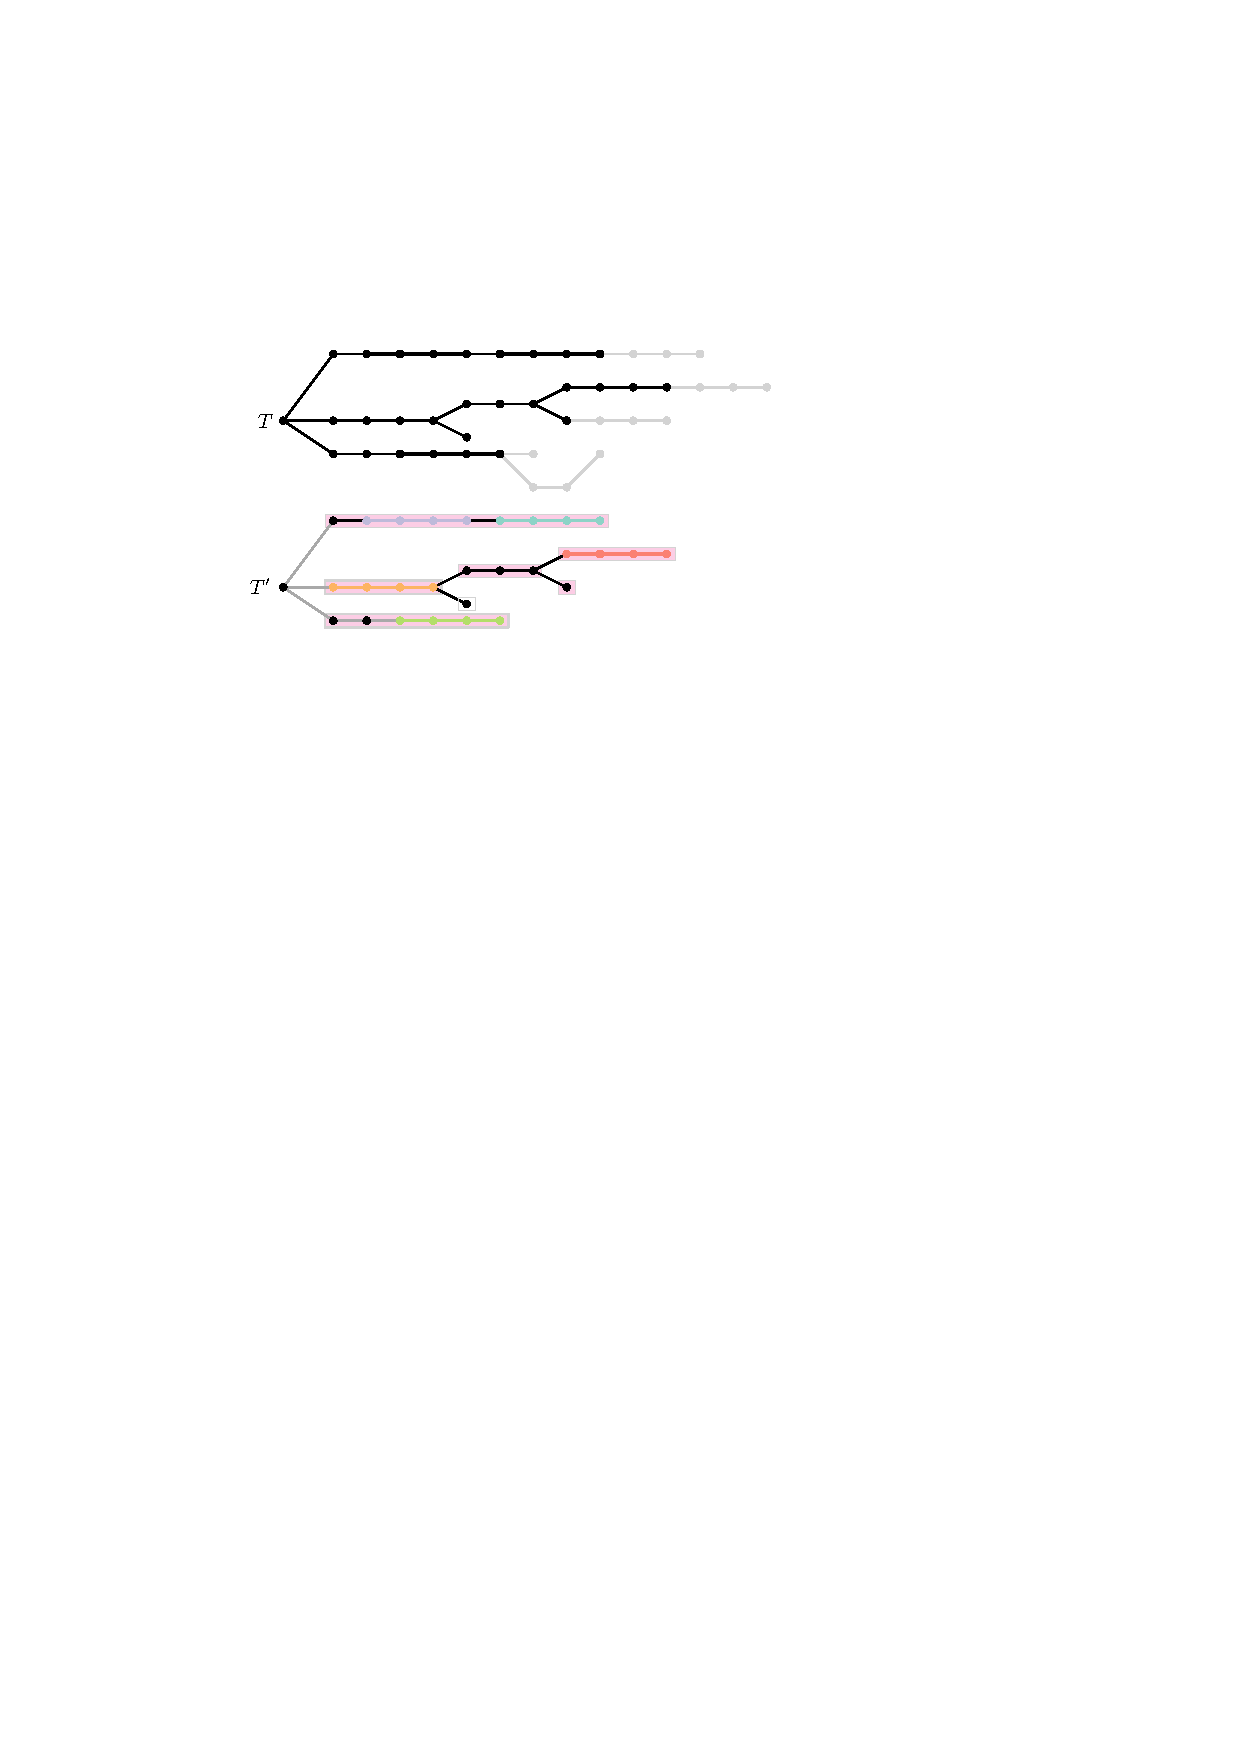
\includegraphics{figs/disjoint-paths}
    \end{center}
    \caption{Finding paths in the tree $T'$ induced by vertices of height at least $p=4$. Note that the figures are drawn so that for each edge, the left vertex is the upper endpoint.} 
    \label{disjoint_p_paths_figs}
  \end{figure}

  Let $S$ be the set of vertices of $T'$ that have two or more children in $T'$.  In any rooted tree, the number of non-root leaves is greater than the number of non-leaf vertices with at least two children\footnote{Let $n_i$ be the number of vertices with $i$ children in a rooted tree $T$. Thus $\sum_{i\geq 0} i n_i=|E(T)|<|V(T)|=\sum_{i\geq 0}n_i$. Hence, the number of non-root leaves 
  $n_0 > \sum_{i\geq 1} (i-1) n_i \geq \sum_{i\geq 2} n_i$, as claimed.}  Therefore, $|S|<|L|\le \tfrac{n}{4p}$.

  For each $v\in S\cup L$, let $P_v$ be the vertical path of maximum length whose lower endpoint is $v$ and that does not contain any vertex in $(S\cup L)\setminus \{v\}$.  Then $\mathcal{P}:=\{P_v:v\in S\cup L\}$ is a partition of $V(T')$ into at most $r:=|S|+|L|\le \tfrac{n}{2p}$ parts, each of which induces a vertical path in $T'$.

  Let $\{P_1,\ldots,P_r\}:=\mathcal{P}$ and, for each $i\in\{1,\ldots,r\}$, let $P'_i$ be a subpath of $P_i$ of order $p\floor{|P_i|/p}$. (So $P'_i$ has order rounded down to a multiple of $p$.)  Then 
  $$\sum_{i=1}^r |P_i'|\ge \sum_{i=1}^r (|P_i|-(p-1)) = |T'| - (p-1)r\ge \tfrac{3n}{4}-\tfrac{n}{2}=\tfrac{n}{4}.$$ 
  For each $i\in\{1,\ldots,r\}$, $P_i'$ can be partitioned into exactly $|P_i'|/p$ vertex-disjoint paths, each of order $p$.  The set $\mathcal{P}'$ of paths obtained this way has size $\ell := \sum_{i=1}^r |P_i'|/p \ge \tfrac{n}{4p}$.  Therefore $T$ contains $\ell$ pairwise vertex-disjoint paths, each of order $p$, where $\ell\ge \tfrac{n}{4p}$.  Except for its lower endpoint, each vertex of a path in $\mathcal{P}'$ has exactly one child in $T$.  This ensures that each path in $\mathcal{P}'$ is either completely related or completely unrelated to any other path in $\mathcal{P}'$.
\end{proof}




% \subsection{A Digression}
%
% As an aside, the question of how large a subdivided star a connected $n$-vertex graph $G$ must contain may be of independent interest.  Almost the same proof used to show \cref{newer_subdivided_star_minor} can be used to show the following lemma.  The only difference in the proof is that the two cases to consider are $i k_i\ge n/H_n$ for some $i\in\{1,\ldots,k+1\}$ or $i k_i < n/H_n$ for all $i\in\{1,\ldots,k+1\}$.
%
% \begin{lem}\label{new_subdivided_star_minor}
%     For every tree $T$ with $n \ge 1$ vertices, there exists integers $\ell$,$p$ with $\ell p \in \Omega(n/\log n)$, a subtree $T'$ of $T$, and disjoint paths $p_1, p_2, ..., p_\ell$ in $T - V(T')$, such that for each $i \in \{1,...,\ell\}$, one endpoint of $p_i$ is adjacent to some vertex in $T'$ and $|V(p_i)| = p$.
% \end{lem}
%
% \begin{proof}
% Consider a sequence of trees $T_0, T_1, ...$, where $T_0:=T$ and, for $i \ge 1$, $T_i$ is the tree obtained from $T_{i-1}$ by removing all vertices of degree at most one. Since any tree with $n \ge 2$ nodes has at least 2 leaves, $|V(T_i)|\le n-2i$ for each $i\le n/2$. Therefore $T_{\floor{n/2}}$ has at most one node and $T_{\floor{n/2}+1}$ is empty. Therefore, there is an index $k \le \floor{n/2}$ such that $T_k$ has at least one vertex and $T_j$ is empty for all $j > k$. For each $i \in \{1,...,k+1\}$, let $k_i$ be the number of vertices in $T_{i-1}$ of degree at most one. We distinguish between two cases:

% \begin{compactenum}[(1)]
%     \item $ik_i \ge n/H_n$ for some $i \in \{1,...,k+1\}$. In this case, $T_{i-1}$ is a tree with $k_i$ vertices of degree at most one.  For $k_i\ge 2$, this means that $T_{i-1}$ has $k_i$ leaves.  Each leaf $v$ of $T_{i-1}$ is a node that, in $T$, is the first node on a path $P_v$, of order $i$, to one of $v$'s leaf descendants in $T$.  The set $\{P_v:\text{$v$ is a leaf $T_{i-1}$}\}$ gives a collection of $\ell:=k_i$ paths, each of order $p=i$.

%     %underline to be replaced by a cref
%     Now, we can take $T'=T_i$. Its then clear that first vertex of each path is adjacent to a vertex in $T'$. Finally, note that these paths are also necessarily disjoint as any two paths that meet would result in a cycle, contradicting that $T$ is a tree.

%     Thus, we have $\ell$ disjoint paths of length $p$, with $\ell p = ik_i \ge n/H_n \ge \Omega(n/\log n)$ and a subtree $T'$ of $T$ such that one endpoint of each of the $\ell$ paths is adjacent to a vertex in $T'$.

%     \item $ik_i < n/H_n$, for each $i \in \{1,...,k+1\}$.  For each vertex $v$ of $T$ there is exactly one value of $i\in\{0,\ldots,k\}$ such that $v$ has degree at most one in $T_i$.
%     Thus, $\sum_{i=1}^{k+1} k_i = n$. Since $ik_i < n/H_n$, we have that  $k_i < n/iH_n$.  Putting these two facts together, we get:
% \[
%     n = \sum_{i=1}^{k+1} k_i < \sum_{i=1}^{k+1} n/iH_n = n/H_n\sum_{i=1}^{k+1}1/i = n H_{k+1}/H_n \le n H_{\floor{n/2}+1}/H_n \le n \enspace ,
% \]
% for any $n\ge 1$.
% This gives a contradiction, so this case does not occur. \qedhere
% \end{compactenum}
% \end{proof}

% We say that a path $P$ in a rooted tree $T$ is \defn{vertical} if it is contained in a single root-to-leaf path in $T$.  Say that a set of paths in $T$ is \defn{unrelated} if the paths are vertex disjoint and no vertex of any path is a $T$-ancestor of a vertex in a different path.    \Cref{new_subdivided_star_minor} shows that any $n$-vertex tree contains an unrelated set of $\ell$ paths, each of size $p$, for some $p\ell \in\Omega(n/\log n)$.  The following lemma shows that this bound is asymptotically tight.\footnote{If $n=h2^{h+1}$, then $2^{h+1}\in \Theta(n/\log n)$.}
%
% \begin{lem}\label{pl_upper_bound}
%     For every integer $h\ge 0$, there exists a rooted tree $T$ with $n:=1+h2^{h+1}$ vertices and such that, if $T$ contains an unrelated set of $\ell$ vertical paths, each of length $p$, then $\ell p\le 2^{h+1}$.
% \end{lem}
%
% \begin{proof}
%   The tree $T$ has a root vertex $v_0$ and each subtree incident to $v_0$ is a path.  These subtrees are grouped into sets $\mathcal{P}_0,\ldots,\mathcal{P}_h$ where each $\mathcal{P}_i$ contains $2^i$ paths, each having $2^{h-i}$ vertices.  It follows from this definition that the number of vertices in $T$ is $n:=1+\sum_{i=0}^h 2^i\cdot 2^{h-i}=1+ (h+1) 2^{h}$.
%
%   Let $\mathcal{P}:= \{P_1,\ldots,P_{\ell}\}$ be an unrelated set of vertical paths in $T$, each having $p$ vertices.
%   % Without loss of generality we may assume that each path in $P$ contains a leaf of $T$.
%   Let $k:=h-\lceil \log_2 p\rceil$ and observe that $2^{h-(k+1)} < p$. Therefore, any path in $\mathcal{P}$ that does not contain $v_0$ does not contain any vertex of $\cup \mathcal{P}_j$ for any $j\ge k+1$ since the number of vertices of each path in $\mathcal{P}_j$ is only $2^{h-j}\le 2^{h-(k+1)} < p$.  Since the paths in $\mathcal{P}$ are unrelated, $\mathcal{P}$ contains at most $2^i$ paths in $\mathcal{P}_i$, for each $i\le k$.  Therefore, $\ell=|\mathcal{P}|\le 1+ \sum_{i=0}^{k} 2^i=2^{k+1}=2^{h+1-\lceil\log_2 p\rceil}\le 2^{h+1}/p$.  Therefore, $\ell p \le 2^{h+1}$.
% \end{proof}
% % T has n vertices.
% % n-1 = size of all stars combined (all vertices but root)
% % = \sum_{i=0}^k (2^i)(n/2^i\logn) + 1 = kn/\log n + k
% % \implies n-1 = k(1 + n/\log n) \implies k = n-1/(1 + n/log n) which solves to k = (n-1)\log n / (n + \log n).
%     % Let $n$ be such that $k = (n-1)\log n/(n + \log n)$ is a positive integer and consider a tree $T$ on $n$ vertices rooted at a vertex $r$ such that, for each $i \in \{0, ..., k\}$, $r$ has a child whose subtree is $S^i = S_{2^i, 1 + n/2^i\log n}$. The choice of $k$ guarantees that these stars contain the remaining $n-1$ vertices.
%
%     % Now, these stars all have the same number of vertices and thus the same subtree rank, but correspond to different choices for the heavy path length rank. Regardless of our choice of path length rank we can find $2^i$ paths of length $n/2^i\log n$ for a total of $n/\log n$ vertices. The additional vertex in each path of the subdivided star guarantees that no two paths of the same length are an ancestor of another.
%
%     % Thus by selecting any of the stars we can satisfy \cref{subdivided_star_minor} with $T'$ consisting of $r$, the root of each star (i.e. every child of $r$), and the paths from the unused stars. The $p_i$'s used are the arms of the selected star $S_{2^i, 1 + n/2^i\log n}$, which all have length $n/2^i\log n$ for a total of $2^in/2^i\log n = n/\log n$ vertices. Finally, its clear that each $p_i$ is adjacent to the root of the selected star, which is in $T'$.
%
%     % To see the upper bound on $\ell p $, Consider that if we want all paths of length $n/2^i\log n$, we cannot choose any paths from stars $S^j$ where $j > i$ as the length of the paths in $S^j$ are at most $n/2^j\log n < n/2^i\log n$..
%     % We can, however, choose all of the paths from any star $S^j$ with $j \le i$. Specifically, we can choose $2^j$ paths from $S^j$ for each $j < i$. This means the total number of vertices among all paths of length $n/2^i\log n$ is
%     % \[(n/2^i\log n)\sum_{j=0}^i2^j = \frac{n}{2^i\log n}(2^{i+1}-1) < 2n/\log n.\]
%
% \subsection{What's Missing}
%
% I think we could get an optimal bound if we can prove the following result:
%
% \begin{conj}[FALSE]\label{too_bold}
%     There exists a constant $\alpha > 0$ such that each tree $T$ contains pairwise unrelated paths $P_1,\ldots,P_r$ with $\sum_{i=1}^r |V(P_i)|\ge \alpha |V(T)|$.
% \end{conj}
%
% \begin{proof}[Disproof of \cref{too_bold}]
%     Let $T_0$ be the $1$-vertex tree.  For $k\ge 1$, $T_k$ is the rooted tree constructed by taking a path $P$ with $2^k$ vertices.  The first vertex of $P$ is the root of $T_k$.  The last vertex of $P$ has two children, each of which is the root of a copy of $T_{k-1}$.  Then $|V(T_k)|=\sum_{j=0}^k 2^j 2^{k-j}=(k+1)2^k$ vertices and has vertex height $h(T_k)=\sum_{j=0}^k 2^{k-j}=2^{k+1}-1$.
%
%     Let $P_1,\ldots,P_r$ be a set of pairwise unrelated paths in $T_k$ where $P_1$ is the longest path and has order $2^p\le |P_1|< 2^{p+1}$.  We claim that $\sum_{j=1}^r |V(P_j)|\le 2^{k+1}-1$. Since $h(T_k)=2^{k+1}-1$, $p\le k$.  The number of vertices of $T_k$ with vertex height $2^p$ is exactly $2^{k-p}$ and $P_1$ contains one of these vertices.  Each of the remain paths is contained in one of the $2^{k-p}-1$ copies of $T_{p}$ not intersected by $P_1$.  By the inductive hypothesis, the total size of all paths contained in one copy of $T_p$ is at most $2^{p+1}-1$.  Therefore, the total size of all paths is at most
%     \begin{align*}
%         \sum_{j=1}^{r}|P_j|
%           & \le |P_1| + (2^{k-p}-1)\cdot (2^{p+1}-1) \\
%           & = |P_1| + 2^{k+1} - 2^{k-p} - 2^{p+1}+ 1 \\
%           & \le 2^{p+1}-1 + 2^{k+1} - 2^{k-p} - 2^{p+1} + 1 \\
%           & = 2^{k+1} - 2^{k-p} \le 2^{k+1}-1 \enspace .
%     \end{align*}
%     This disproves the conjecture because if we define $n:=|V(T_k)|=(k+1)2^{k}$ then $2^{k+1}-1\in O(n/\log n)$.  \pat{We should use this example to prove \cref{pl_upper_bound} instead of what's there now.}
% \end{proof}
%
%
% June 15: 16:21:  I now know what to do.  In \cref{star_times_star}, below, we don't need two subdivided stars.  It's sufficient to have a product of the form $T\boxprod S_{\ell,p}$ where $p^2\ell\in\Omega(n)$ and $T$ is a tree that contains $\Omega(n/p^2)$ pairwise-disjoint paths, each of length $p$.

\subsection{The Product of Two Special Trees}

% We now complete the second part of our proof, by showing that the two trees guaranteed by \cref{subdivided_star_minor} and

\begin{lem}\label{star_times_star}
  Let $s,p\ge 1$ be integers, let $\ell:=5s^2$, and let $T$ be a rooted tree that contains $s^2$ pairwise-disjoint vertical paths, each of order $6p$ such that any pair of these paths is either completely related or completely unrelated.  Then $\gm(T\boxprod S_{\ell,2p})\ge sp$.
\end{lem}

\begin{proof}
  Recall that $S_{\ell,2p}$ has vertex set $\{v_0\}\cup\{v_{i,j}:(i,j)\in \{1,\ldots,\ell\}\times\{1,\ldots,2p\}\}$. For each $i\in\{1,\ldots,\ell\}$, let $A_i=S_{\ell,2p}[\{v_{i,1},\ldots,v_{i,2p}\}]$ denote the $i$th \defn{arm} of $S_{\ell,2p}$, which is a path of order $2p$.  Let $P_1,\ldots,P_{s^2}$ be pairwise vertex-disjoint paths in $T$, each of order $6p$, each pair of which is either completely related or completely unrelated.  For each $i\in\{1,\ldots,s^2 \}$, let $P_i:= p_{i,1},\ldots,p_{i,6p}$ where $p_{i,1}$ is the upper endpoint of $P_i$. 
  Let $T_0:=T\boxprod \{v_0\}$.  For each $i\in\{1,\ldots,\ell\}$ let $T_i:=T\boxprod A_i$, for each $j\in \{1,\ldots,p\}$ let $T_{i,j}:=T\boxprod \{v_{i,j}\}$, for each $k\in\{1,\ldots,s^2\}$ let $P_{k,i}:=P_k\boxprod A_i$ and $P_{k,i,j}:=P_k\boxprod \{v_{i,j}\}$.

  Refer to \cref{product_fig}. 
  Consider $T_i$ for some $i\in\{1,\ldots,\ell\}$. For visualization purposes, it is helpful to organize $T_i$ into $2p$ rows $T_{i,1},\ldots,T_{i,2p}$.  For each $j\in\{1,\ldots,2p-1\}$, $T_{i,j}$ and $T_{i,j+1}$ are `adjacent' in the sense that each vertex $(a,v_{i,j})\in V(T_{i,j})$ is adjacent to $(a,v_{i,j+1})\in V(T_{i,j+1})$.  We then organize $T_1,\ldots,T_{\ell}$ into a sequence of blocks. These blocks are independent in the sense that there is no edge between $T_{i}$ and $T_j$ for any $i\neq j$.  Moreover, there is an additional row $T_0$ that is adjacent to the first row, $T_{i,1}$, of each block $T_i$.

  \begin{figure}[ht]
    \begin{center}
      \includegraphics[page=4]{figs/product}
    \end{center}
    \caption{Visualizing the product in \cref{star_times_star}}
    \label{product_fig}
  \end{figure}

  Refer to \cref{grid_partition}.  We will construct a model of $\boxplus_{sp}$. 
  We partition this model into $s^2$ subgrids each of which is isomorphic to $\boxplus_p$.  Therefore, we need $s^2$ such subgrids $G_1,\ldots,G_{s^2}$. The branch sets of each subgrid $G_i$ will include a $p\times p$ grid within the $6p\times 2p$ grid $P_{i,i}$ (which is contained in the block $T_i$).  The additional row $T_0$ will allow us to extend the branch sets of the $4p-4$ boundary vertices of the $G_i$ into $T_{i'}$ for any $i'$ and from there they can be extended so that they are adjacent to any other subgrid $G_j$.

  \begin{figure}
    \begin{center}
      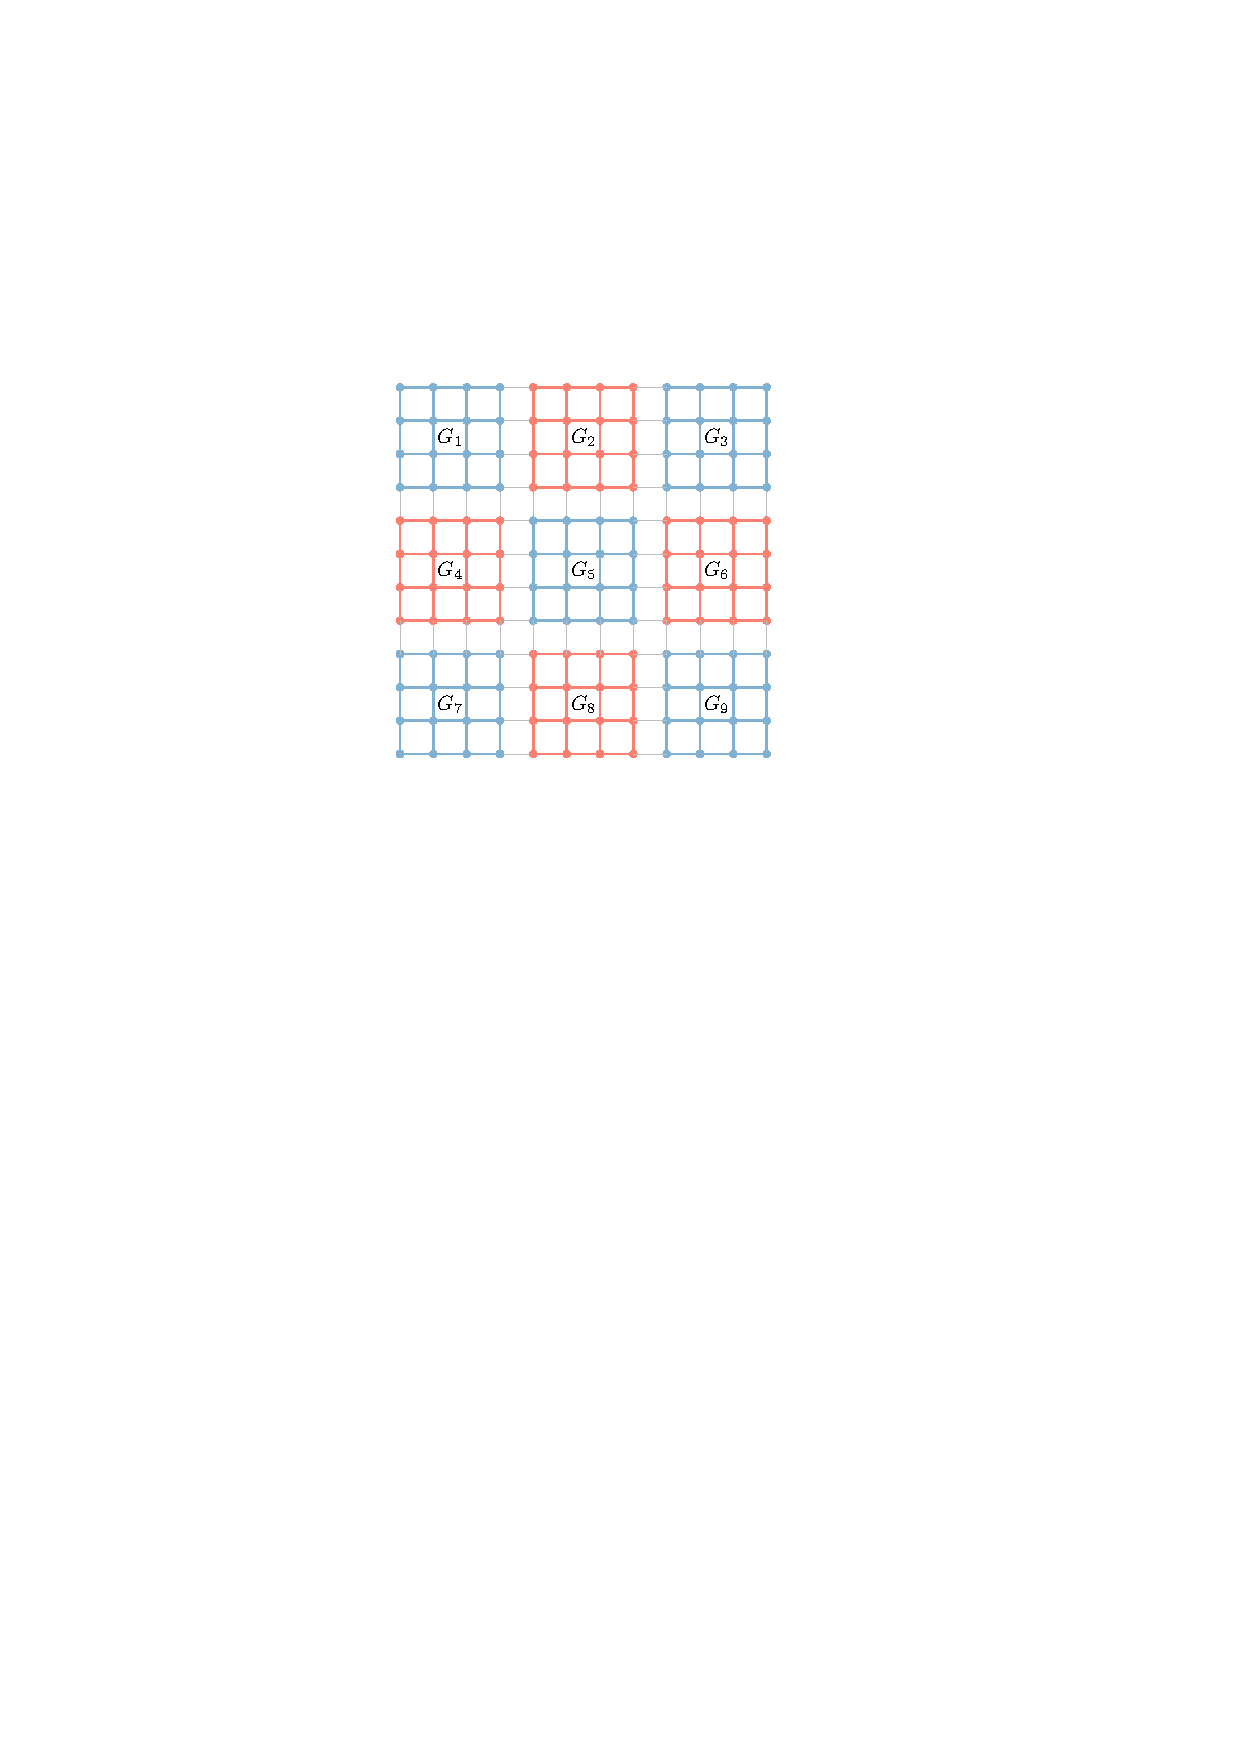
\includegraphics{gridlayout}
    \end{center}
    \caption{The $sp\times sp$ grid can be partitioned into $(sp/p)^2 = s^2$ subgrids, each of which is a $p\times p$ grid. (The case $sp=12$ and $p=4$ is shown here.)}
    \label{grid_partition}
  \end{figure}

  \begin{figure}[H]
    \begin{center}
      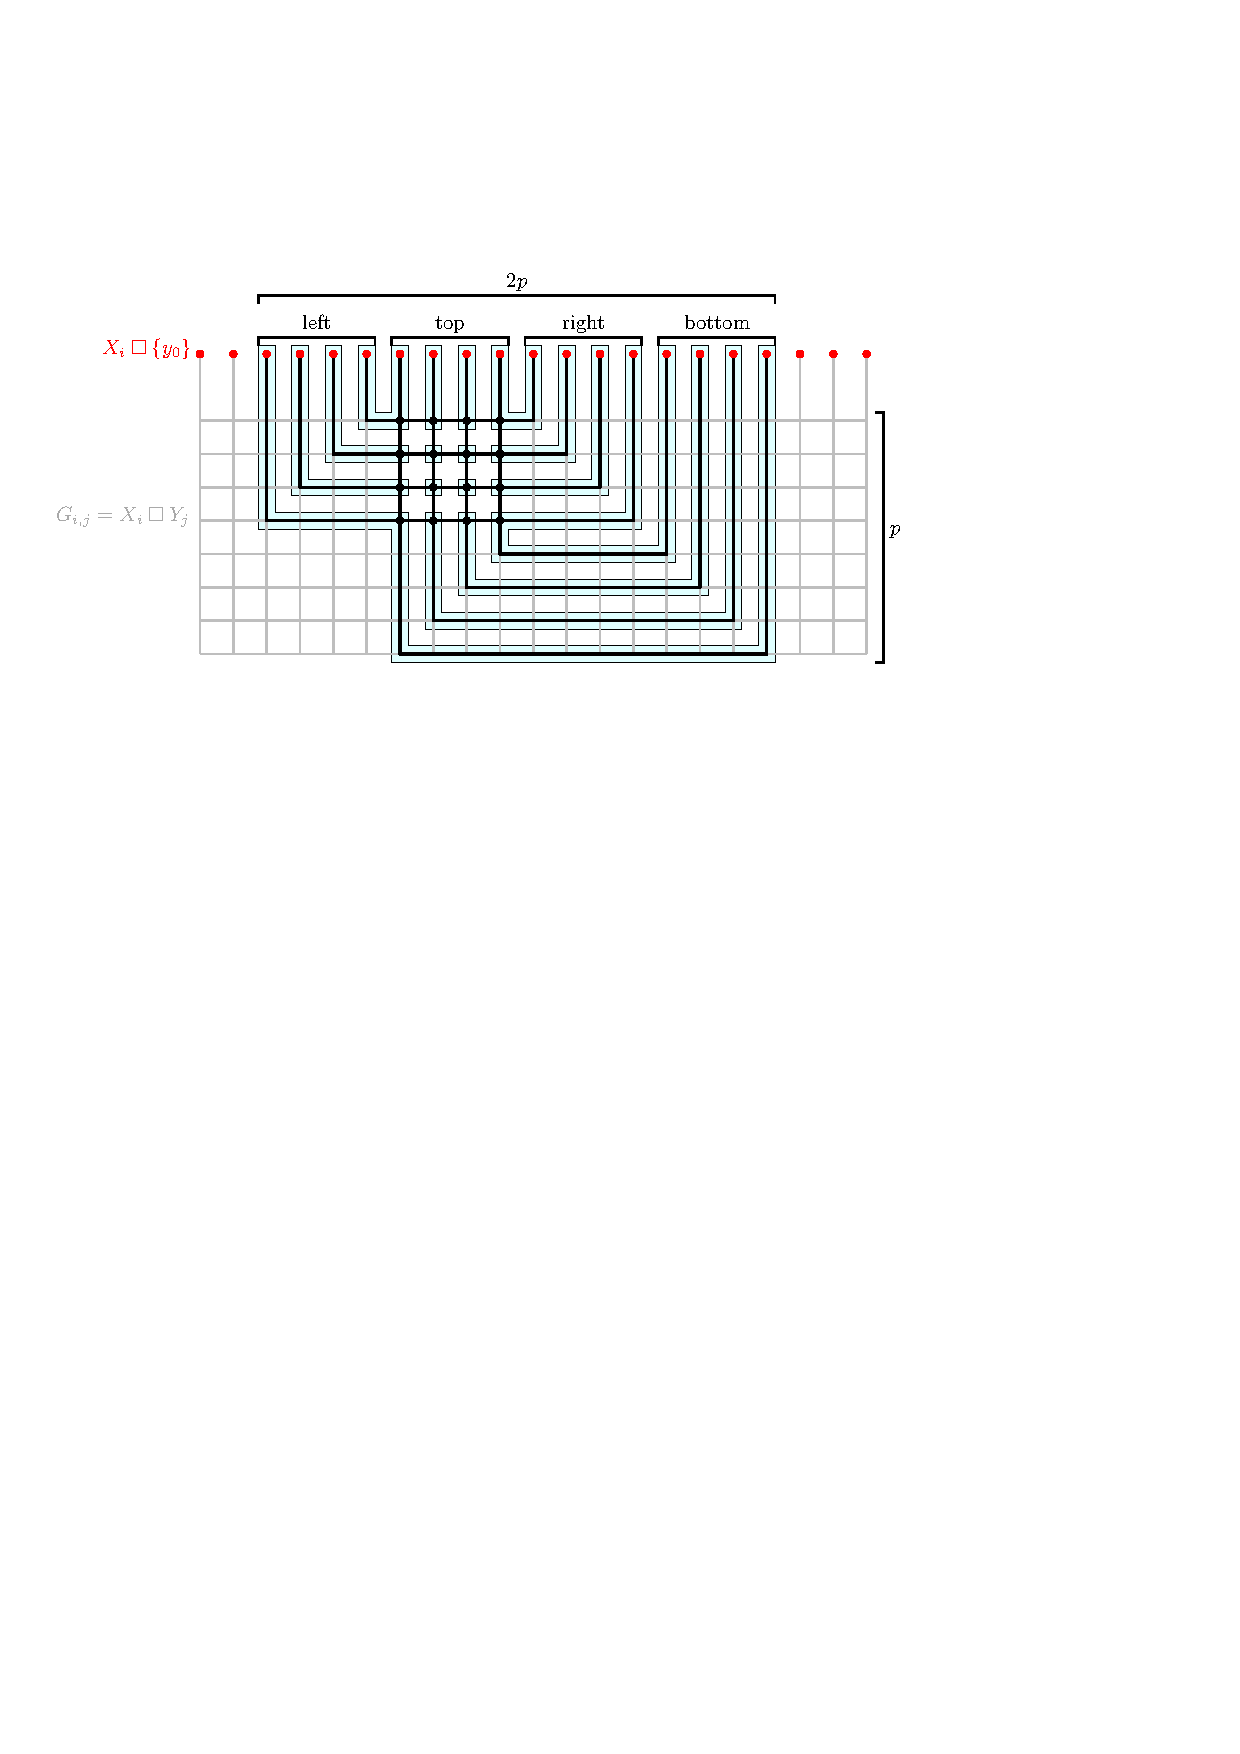
\includegraphics[width=\textwidth]{subgrid}
    \end{center}
    \caption{One of the $p\times p$ subgrids used in the proof of \cref{star_times_star}.}
    \label{subgrid}
  \end{figure}

  Refer to \cref{subgrid}. To construct the branch sets for $G_i$ we start with a $p\times p$ subgrid in $P_{i,i}$ whose top row is $(p_{i,p+1},v_{i,1}),\ldots,(p_{i,2p},v_{i,1})$.  This subgrid has $4p-4$ `boundary' vertices, four of which are `corner' vertices. As illustrated in \cref{subgrid}, we create $4p$ disjoint paths in $P_{i,i}$ from the boundary vertices to $P_{i,i,1}$.  We then add one vertex of $P_{i,0}$ to each path.  In this way, the first $4p$ vertices of the path $P_{i,0}$ are partitioned into four subpaths, each of size $p$ corresponding to edges coming out of the left, top, right, and bottom of boundary of $G_i$.  The final $2p$ vertices of $P_{i,0}$ are not yet used (though we may add them to the branch sets of some boundary vertices later).


  Our model is not yet complete.  At this point, it is a model of a graph that consists of $s^2$ components, each of which is a $p\times p$ grid.  At this point, the vertices in our (not yet-complete) model are all contained in $T_0,T_1,\ldots,T_{s^2}$ and, for each $i\in\{1,\ldots,s^2\}$, the branch sets of vertices in $G_i$ are contained $P_{i,i}\cup P_{i,0}\subseteq T_{i}\cup P_{i,0}$.  This still leaves the vertices of $T_{s^2+1},\ldots,T_{5s^2}$ unused.  We will use these to extend the branch sets of vertices on the boundary of each subgrid $G_i$ to create the required adjacencies.  For each $i\in\{1,\ldots,s^2\}$, the vertices of $T_{s^2+4i-3},\ldots,T_{s^2+4i}$ will be reserved for the branch sets of $G_i$.

  First, suppose that $G_i$ is a subgrid that is immediately to the right of some subgrid $G_j$, so that the left boundary of $G_i$ is adjacent to the right boundary of $G_j$.  We will extend the branch sets for vertices on the left boundary of $G_i$ so that they become adjacent to the branch sets for vertices in the right boundary of $G_j$. Let $x_1,\ldots,x_p$ be the vertices on the left boundary of $G_i$, ordered from top to bottom and, for each $k\in\{1,\ldots,p\}$, let $x_k':=p_{i,k}$ so that $(x_k',v_0)$ is already included in the branch set for $x_k$.  Let $y_0,\ldots,y_p$ be the vertices on the right boundary of $G_j$, ordered from top to bottom and, for each $k\in\{1,\ldots,p\}$, let $y_k':=p_{j,2p+k}$ so that $(y_k',v_0)$ is already included in the branch set of $y_k$. There are two cases to consider.  (We strongly urge the reader to refer to \cref{straight,reverso}.)

% \david{I think it will help the reader if the text describing Figure 6 appears on the same page as the figure. So I have added a newpage here temporarily. I suggest when the paper is finished we play with the margins to remove this big whitespace.}
\newpage

  \begin{itemize}
    \item $P_i$ and $P_j$ are completely related (see \cref{straight}): We will extend the branch sets of $x_1,\ldots,x_p$ into $T_{s^2+4i-3}$.  For each $k\in\{1,\ldots,p\}$, we extend the branch set of $x_k$ by adding the path
    \[
      (x_k',v_{s^2+4i-3,1}),\ldots,(x_k',v_{s^2+4i-3,k}) \enspace ,
    \]
    the path in $T_{s^2+4i-3,k}$ from $(x_k',v_{s^2+4i-3,k})$ to $(y_k',v_{s^2+4i-3,k})$, and the path
    \[
      (y_k',v_{s^2+4i-3,k}),\ldots,(y_k',v_{s^2+4i-3,1}) \enspace .
    \]
    The first vertex $(x_k',v_{s^2+4i-3,1})$ of this path is adjacent to $(x_k',v_0)$, which ensures that the branch set for $x_k$ is connected.  The last vertex $(y_k',v_{s^2+4i-3,1})$ is adjacent to $(y_k',v_0)$ which ensures that the branch sets for $x_k$ and $y_k$ are adjacent.

    \begin{figure}[t]
      \begin{center}
      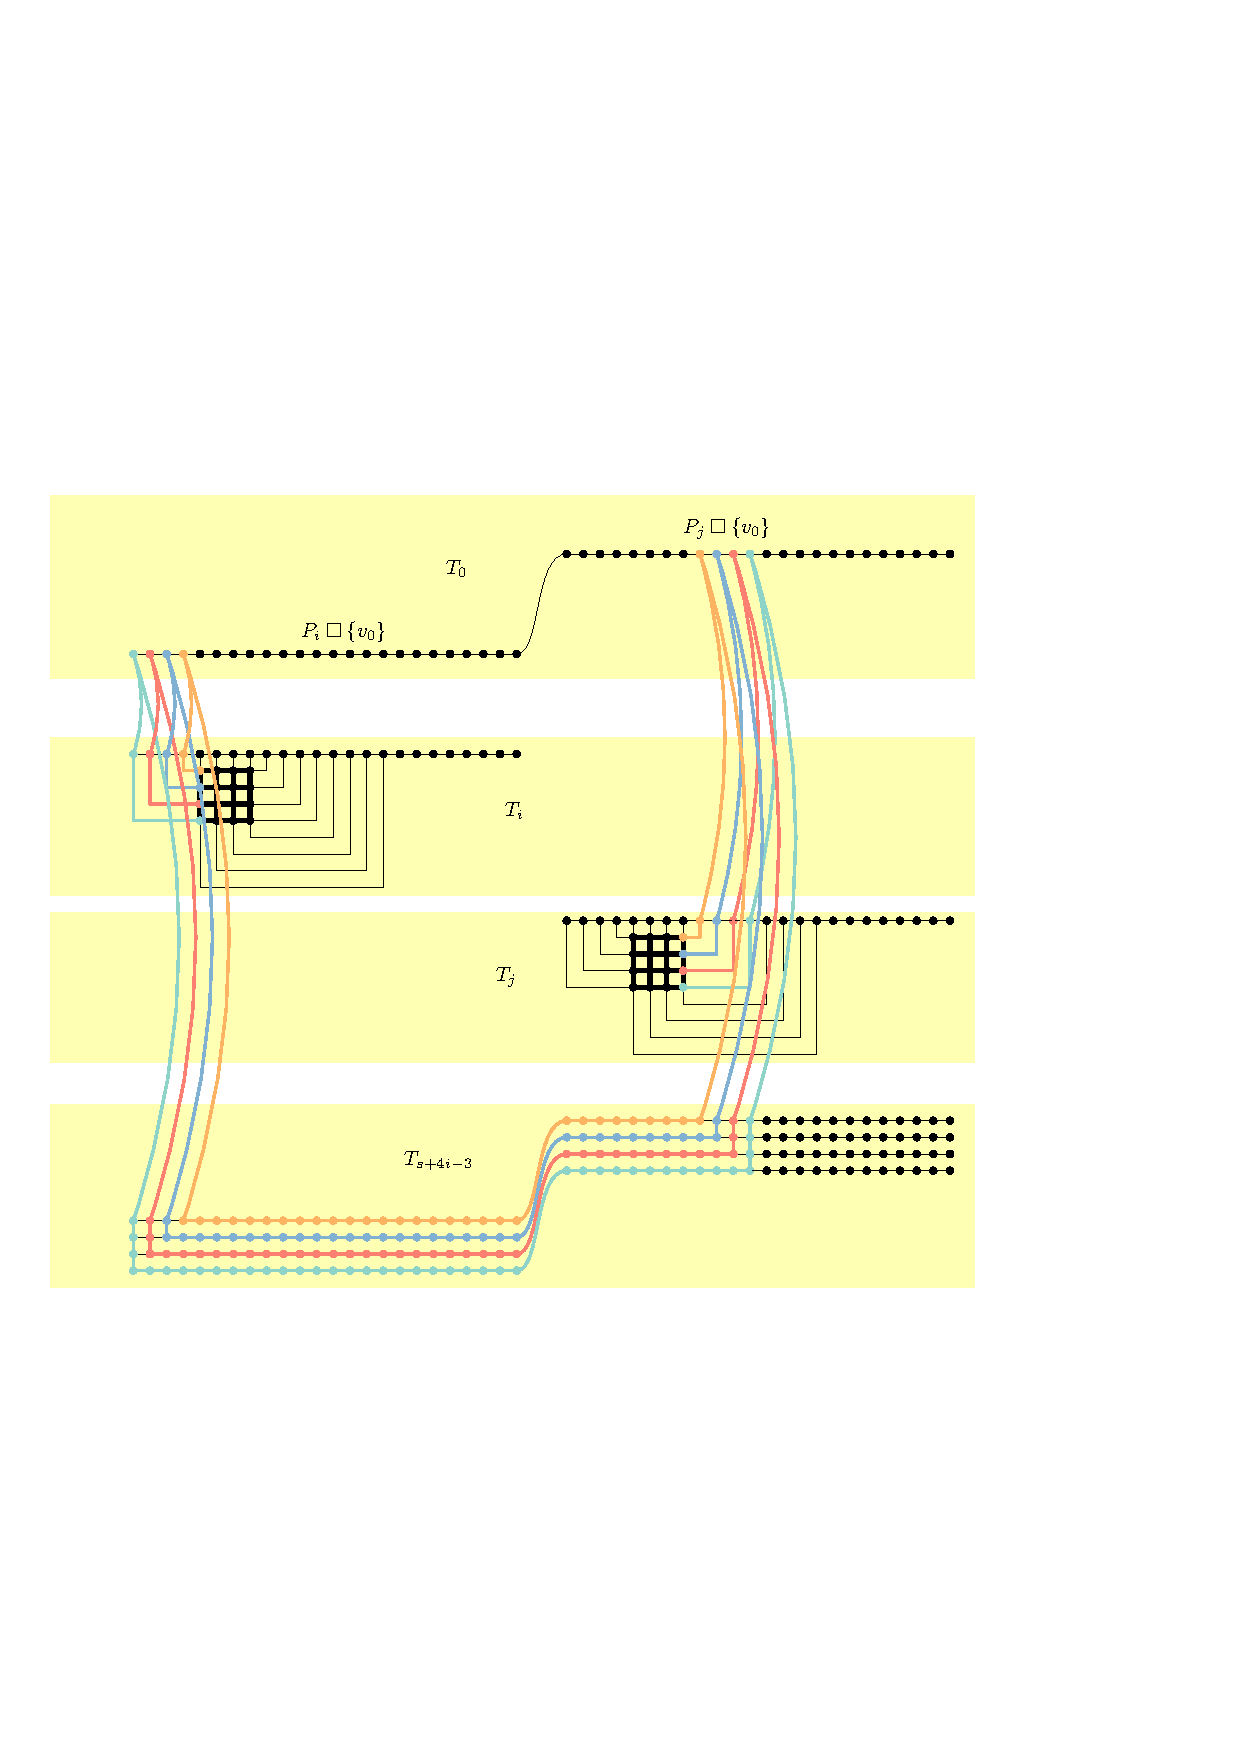
\includegraphics[scale=0.9]{figs/straight}
      \end{center}
      \caption{Connecting the left side of $G_i$ to the right side of $G_j$ when $P_i$ and $P_j$ are completely related.}
      \label{straight}
    \end{figure}

    \newpage


    \item $P_i$ and $P_j$ are completely unrelated (see \cref{reverso}): We will extend the branch sets of $x_1,\ldots,x_k$ into $T_{s^2+4i-3}$ and $T_{s^2+4i-2}$. To make the connections between these two blocks we will use an additional $p$ vertices of $P_{i,0}$.  The need for a second block in this case is due to the fact that the obvious paths in $T_{s^2+4i-3}$ that were used in the previous case would either intersect each other or reverse the order of connections so that the top-left vertex of $G_i$ would become adjacent to the bottom-right vertex of $G_j$. Routing these paths through two trees allows us to make the connections in the right order using pairwise vertex-disjoint paths.

     \begin{figure}[H]
      \begin{center}
        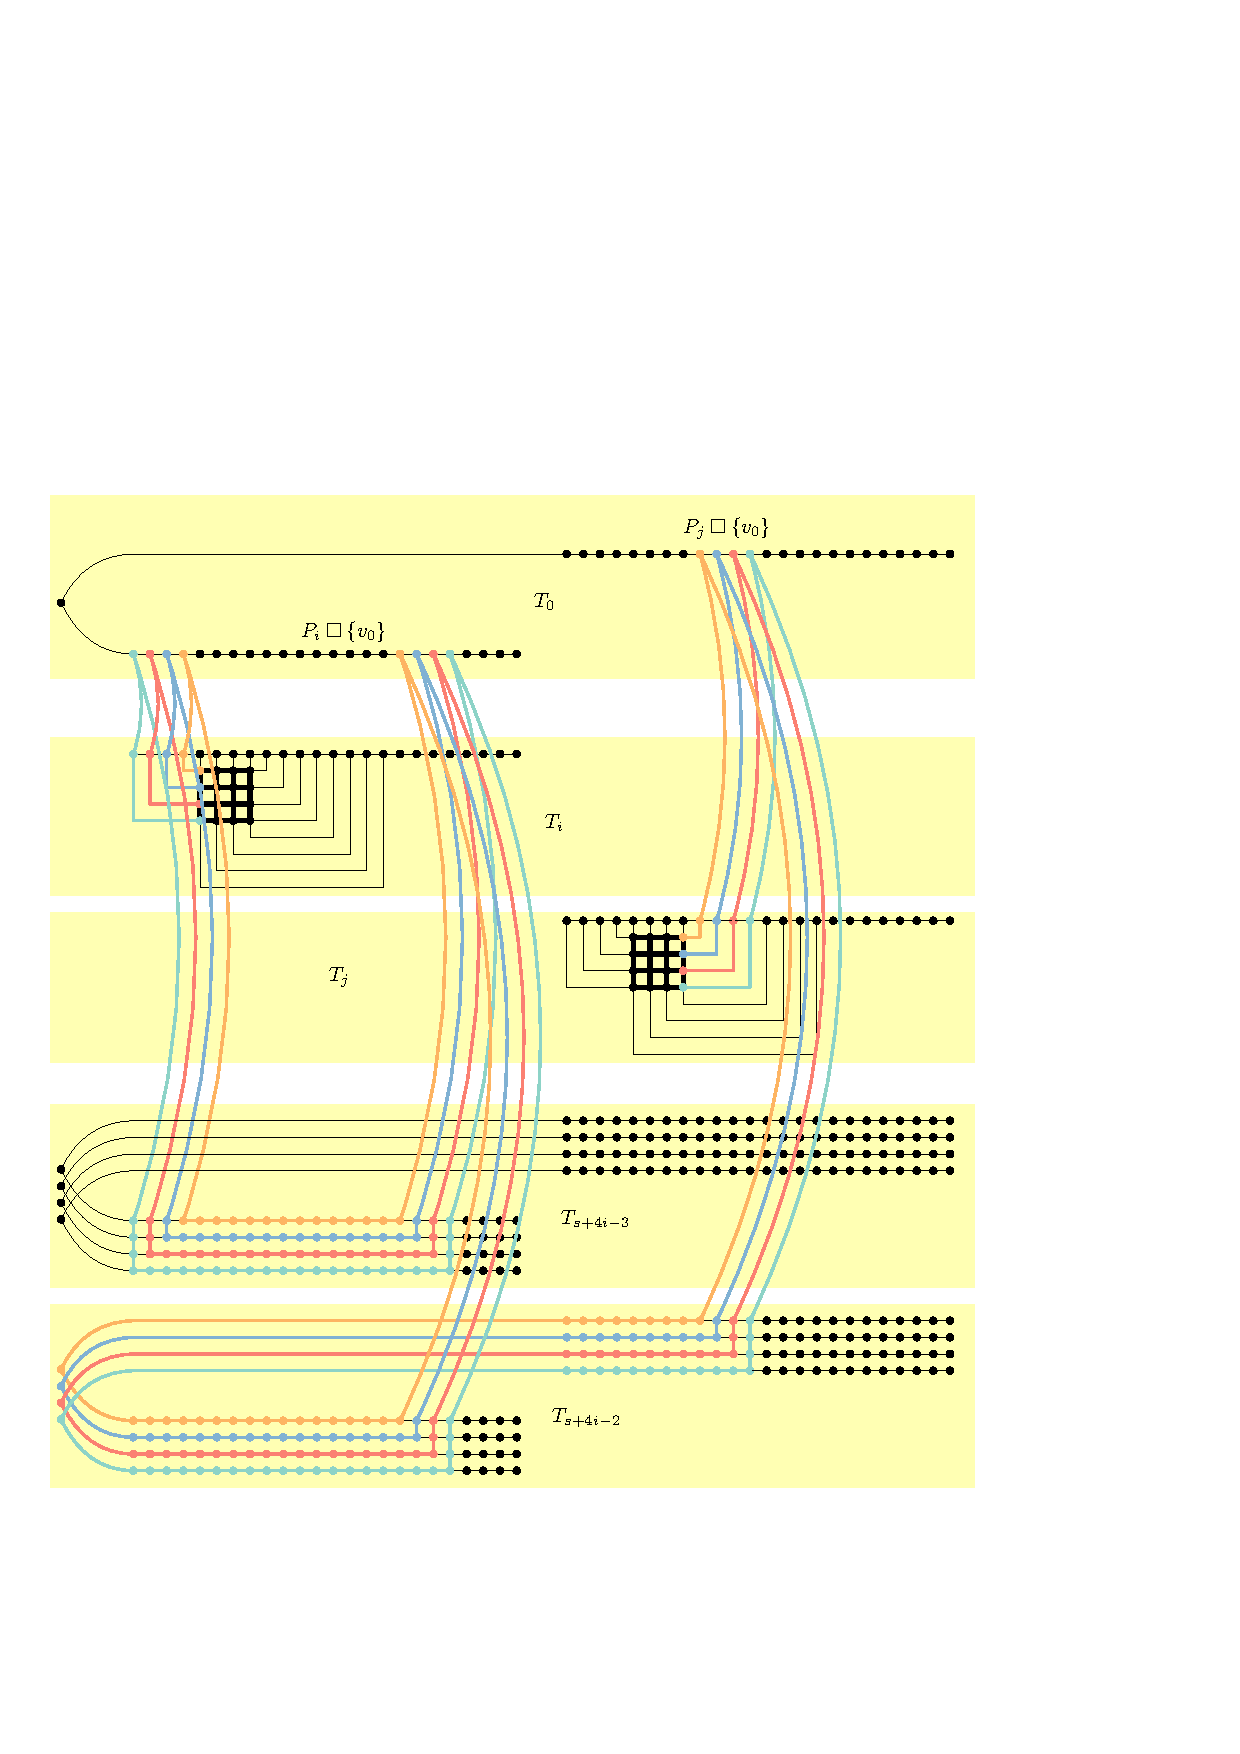
\includegraphics[scale=0.9]{figs/reverso}
      \end{center}
      \caption{Connecting the left side of $G_i$ to the right side of $G_j$ when $P_i$ and $P_j$ are completely unrelated.}
      \label{reverso}
    \end{figure}

    For each $k\in\{1,\ldots,p\}$ we extend the branch set of $x_k$ by adding the path,
    \[
      (x_k',v_{s^2+4i-3,1}),\ldots,(x_k',v_{s^2+4i-3,k}) \enspace ,
    \]
    the path in $T_{s^2+4i-3,k}$ from  $(x_k',v_{s^2+4i-3,k})$ to $(p_{i,5p-k+1},v_{s^2+4i-3,k})$, the path
    \[
      (p_{i,5p-k+1},v_{s^2+4i-3,k}),\ldots,(p_{i,5p-k+1},v_{s^2+4i-3,0}),(p_{i,5p-k+1},v_{s^2+4i-2,1}),\ldots,(p_{i,5p-k+1},v_{s^2+4i-2,k})
    \]
    the path in $T_{s^2+4i-2,k}$ from $(p_{i,5p-k+1},v_{s^2+4i-2,k})$ to $(y_k',v_{s^2+4i-2,k})$ and finally the path
    \[
      (y_k',v_{s^2+4i-3,k}),\ldots,(y_k',v_{s^2+4i-3,1}) \enspace .
    \]
    As in the previous case, the first vertex of this path ensures that the branch set for $x_k$ is connected and the last vertex ensures that the branch sets of $x_k$ and $y_k$ are adjacent.
  \end{itemize}


  So far, our model now models every horizontal grid edge but does not yet include the vertical edges between $p\times p$ subgrids.  We now sketch how these can be included.  Suppose that the subgrid $G_i$ is directly below the subgrid $G_j$.  Let $x_1,\ldots,x_p$ be the top boundary of $G_i$ ordered so that $x_1$ is the the leftmost vertex and $x_p$ is the rightmost.  For each $k\in\{1,\ldots,p\}$, let $x_k':=(p_{i,p+k})$ so that the branch set of $x_k$ includes $x_k'$.  Let $y_1,\ldots,y_p$ be the bottom boundary of $G_j$ ordered so that $y_1$ is the the leftmost vertex and $y_p$ is the rightmost.  For each $k\in\{1,\ldots,p\}$, let $y_k':=(p_{j,4p-k+1})$ so that the branch set of $y_k$ includes $y_k'$.  Observe that $x_1',\ldots,x_p'$ occur in order along $P_{i}$ but $y_1',\ldots,y_k'$ occur in reverse order along $P_j$.  The effect of this is to reverse the two cases that appear above, so that the straightforward case occurs when $P_i$ and $P_j$ are completely unrelated and the more complicated case occurs when they are completely related.  Otherwise, the process of growing the branch sets for $x_1,\ldots,x_p$ is the same except that the vertices used to grow these new branch sets are contained in $T_{s+4i-1}$, $T_{s+4i}$, and $(p_{i,5p+1},v_0),\ldots,(p_{i,6p},v_0)$.  This ensures that these branch sets do not reuse vertices that are used to make $G_i$ adjacent to the neighbour on its left.

  Checking that the resulting collection of branch sets is indeed a model of the $r\times r$ grid is straightforward; both the disjointedness of the branch sets and the required adjacencies are guaranteed by the construction.
\end{proof}

We now establish our lower bound on the largest grid minor in a graph product:

\begin{thm}\label{lower_bound}
  If $G_1$ and $G_2$ are connected graphs each having at least $n\ge 1$ vertices, then $$\gm(G_1\boxprod G_2)\in\Omega(\sqrt{n}).$$
\end{thm}

\begin{proof}
  For each $b\in\{1,2\}$, let $T_b$ be a tree contained in $G_b$ and having exactly $n$ vertices (which can be constructed by successively deleting leaves starting with a spanning tree of $G_b$).  
  For each $b\in\{1,2\}$, let $p_b=\min\{i: n_i(T_b)\ge \tfrac{3n}{2(\pi i)^2}\}$.  (This is well-defined since, otherwise $n=\sum_{i=1}^\infty n_i(T_b) < \sum_{i=1}^\infty \tfrac{3n}{2(\pi i)^2} = \frac{n}{4}$.)  Without loss of generality, assume $p_2 \le p_1$ and let $\ell:=\ceil{\tfrac{3n}{2(\pi p_2)^2}}$. By \cref{same_height_unrelated}, $S_{\ell,p_2}\preceq T_2\preceq G_2$.  If $p_2 \le 5$ then $\ell > \frac{3n}{50\pi^2}\in\Omega(n)$ and by \cref{anything_times_star} $K_{\ell}\preceq G_1 \boxprod S_\ell$.
  Since $\boxplus_{\sqrt{\ell}}\preceq K_{\ell}$, this implies that $\gm(G_1\boxprod G_2)\ge \sqrt{\ell}=\Omega(\sqrt{n})$ and we are done, so we may assume that $p_2\ge 6$. Let $p:=\floor{p_2/6}\ge 1$.

  Since $p_1\ge p_2$, $n_i(T_1)\le \tfrac{3n}{2(\pi i)^2}$ for all $i\in\{1,\ldots,p_2\}$.  Therefore, \cref{disjoint_p_paths} implies that $T_1$ contains at least $n/4p_2$ pairwise disjoint paths $P_1,\ldots,P_{\ceil{n/4p_2}}$, each of length $p_2\ge 6p$, such that each pair of paths is either completely related or completely unrelated.  Let
  \[
    s:=\floor{\min\{\sqrt{\ell/5}, \sqrt{n/4p_2}\}} = \Theta(\sqrt{n}/p)
  \]
  so that $\ell \ge 5s^2$ and $\ceil{n/4p_2}\ge s^2$.  By \cref{star_times_star}, $\gm(T_1 \boxprod S_{\ell,6p}) \ge sp=\Theta(\sqrt{n})$.  The lemma now follows from \cref{minor_product}, the fact that $T_1\preceq G_1$, and the fact that $S_{\ell,6p}\preceq S_{\ell,p_2}\preceq G_2$.
  %
  %
  %
  %
  %   \pat{We don't immediately get our result from \cref{star_times_star} because $p=\min\{p_1,p_2\}$.  To see this, consider the case where $p_1=1$, $\ell_1=n$, $p_2=\log n$ and $\ell_2=n/\log^2 n$.  Then $p=1$ and $N=p_2\ell_2=n/\log n$ so \cref{star_times_star} only guarantees that $\gm(G_1\boxprod G_2)=\Omega(\sqrt{p N})=\Omega(\sqrt{n/\log n})$.  Of course, \cref{anything_times_star} handles this, but....}
  %
  % Right now, the best argument I can think of is to branch on the value of $p$.  Apply \cref{newer_subdivided_star_minor} to each of $G_1$ and $G_2$ and suppose that $p_1< p_2$.  If $p:=p_1 < \sqrt{\log n}$ then use \cref{anything_times_star} to deduce that $G_1\boxprod G_2\succeq K_{n/p}\succeq K_{n/\sqrt{\log n}}\succeq \boxplus_{\sqrt{n}/\log^{1/4} n}$, so $\gm(G_1\boxprod G_2)=\Omega(\sqrt{n}/\log^{1/4} n)$.  Otherwise, apply \cref{new_subdivided_star_minor} to $G_2$ to deduce that $G_2\succeq S_{\ell_2,p_2}$ with $\ell_2p_2 \ge n/\log n$ (and $p_2\ge \log^{1/4} n$?).  Then apply \cref{star_times_star} to deduce that $\gm(G_1\boxprod G_2)=\Omega(\sqrt{p\ell_2p_2}) \ge \sqrt{n/\sqrt{\log n}}=\Omega(n/\log^{1/4} n)$.
  % Let $\ell = \min\{\ell_1, \ell_2\}$ and $p = \min\{p_1, p_2\}$. Then, by Lemma~\ref{star_times_star}, $\gm(S_{\ell_1,p_1}\boxtimes S_{\ell_2,p_2})\in\Omega(\sqrt{pN}) = \Omega(\sqrt{\ell p^2}) = \Omega(\sqrt{n})$. Since $S_{\ell_b,p_b}\preceq T_b\preceq G_b$ for each $b\in\{1,2\}$, the result follows from two applications of Observation~\ref{minor_product}.
\end{proof}


Our next result completes the relationships between grid minors and treewidth in products of trees.  

\begin{thm}\label{quadratic_grid_minor}
    For any two trees $T_1$ and $T_2$, 
    \[
\gm(T_1\boxprod T_2) \leq
\gm(T_1\boxtimes T_2) \leq \tw(T_1\boxtimes T_2) \in O(\gm(T_1\boxprod T_2)^2)
 \enspace .
\]
\end{thm}


\begin{proof}
    First note that $\gm(T_1 \boxprod T_2) \le \gm(T_1 \boxtimes T_2)$ since  
    $T_1 \boxprod T_2 \subseteq T_1 \boxtimes T_2$. \eqref{tw_gte_gm} shows that $\gm(T_1 \boxprod T_2) \le \tw(T_1\boxprod T_2)$, and so all that remains is to show $\tw(T_1\boxprod T_2) \in O(\gm(T_1 \boxprod T_2)^2)$.
    
    Let $n_1:=|V(T_1)|$, let $n_2:=|V(T_2)|$, and assume without loss of generality that $n_1\le n_2$.  Let $T_2$ be rooted at an arbitrary vertex.  Then $T_1\boxtimes T_2$ has a tree decomposition $\mathcal{T}:=(B_x:x\in V(T_2))$ where $B_x$ contains $V(T_1)\times\{x\}$ and, if $x$ has parent $y$, then $B_x$ also contains $V(T_1)\times\{y\}$.  This decomposition has width at most $2n_1-1$, so $\tw(T_1\boxtimes T_2)\le 2n_1-1$.  By \cref{lower_bound}, $c\gm(T_1\boxprod T_2) \ge \sqrt{2n_1}$ for some fixed positive constant $c$. 
    Therefore, 
    \[
       (c\gm(T_1\boxprod T_2))^2 \ge 2n_1 > \tw(T_1\boxtimes T_2) \enspace . \qedhere
    \]
\end{proof}

% \pat{Can we strengthen \cref{quadratic_grid_minor} so that it applies to any graphs $G_1$ and $G_2$?  Answer: Not without improving the grid-minor theorem.  The proof of \cref{quadratic_grid_minor} does prove that $\tw(G\boxtimes T)\in O(\gm(G\boxtimes T))$ when $G$ is any graph, $T$ is a tree, and $|V(G)|\le |V(T)|$. More generally, it works when the bigger graph, $G_2$, has bounded treewidth.} 


\section{Upper Bound}\label{C}


This section proves upper bounds of the form, $\gm(G)\in O(\sqrt{n})$, where $G$ is the product of various $n$-vertex graphs, as mentioned in \cref{A}.

% \david{Is there any reason to include 
% \cref{upper_bound} when it is implied by \cref{StarTreeUpperBound} below?}

% \begin{lem}\label{upper_bound}
%   $\gm(S_n\boxtimes P_n)\le \sqrt{5n}+4$
% \end{lem}

% \begin{proof}
% \david{this proof never uses that $S_n$ has $n$ leaves, it could be any star.}
%   Suppose that $S_n\boxtimes P_n$ contains a $\boxplus_k$ minor. We will prove that $k\le\sqrt{5n}+4$. Let $\mathcal{M}:=(B_x:x\in V(\boxplus_k))$ be a model of $\boxplus_k$ in $G$ and let $x_0, \dots x_n$ be the vertices of $S_n$, with $x_0$ being the root.  We say that a branch set $B_x$ of $\mathcal{M}$ is \defn{rooty} if $(x_0,y)\in V(B_x)$ for some $y\in V(P_n)$ and $B_x$ is \defn{rootless} otherwise.  Clearly, the number of rooty parts in $\mathcal{M}$ is at most $n$.

%   Observe that each rootless part $B_x$ of $\mathcal{M}$ is a single path $(x_i,y_j),\ldots,(x_i,y_{j+\ell})$.  There are at most two other rootless parts [one containing $(x_i,y_{j-1})$ and one containing $(x_i,y_{j+\ell+1})$] adjacent to $B_x$. If $x$ is a vertex of degree at least $3$ in $\boxplus_k$, then $B_x$ must be adjacent to at least one rooty part $B_y$ such that $xy$ is an edge of $\boxplus_k$; we call this a \defn{rooty-rootless adjacency}. The grid $\boxplus_k$ has $k^2-4$ vertices of degree at least $3$. The model $\mathcal{M}$ has $k^2$ parts and at most $n$ of these are rooty, so there are at least $k^2-n$ rootless parts.  Therefore, there are at least $k^2-4-n$ rooty-rootless adjacencies. Since $\boxplus_k$ has maximum degree 4, each rooty part of $\mathcal{M}$ can account for at most four of these adjacencies, 
%  so $k^2-4-n \le 4n$, proving the result.\footnote{We could actually prove a bound of $\approx\sqrt{2n}$ by using the fact that most rootless parts need to be adjacent to two rooty parts. \david{I think this is worth doing, since 2 would be best possible.}}
% \end{proof}

% \cref{anything_times_star} implies that $\tw(S_n\boxprod P_n)\in\Omega(n)$. With this, 
% %~\cite{WoodJGT13}\david{\cref{anything_times_star} implies $\tw(S_n\boxprod P_n)\geq \tw(K_n)=n-1$, so I suggest we cite \cref{anything_times_star} here rather than \cite{WoodJGT13}},
% \cref{upper_bound} has the following consequence, which matches the upper bound in \cref{quadratic_grid_minor}. 
% % \pat{Give a reference or explain the bramble that proves $\tw(S_n\boxprod P_n)\ge n$.}

% \begin{cor}\label{quadratic_grid_minor_cor}
%     There exists $c>0$ such that,
%     for every $n\ge 1$ there exists two trees $T_1$ and $T_2$ such that $\tw(T_1\boxprod T_2)\ge n \ge c (\gm(T_1\boxtimes T_2))^2$.
% \end{cor}

% \david{I have removed this paragraph} As a warm-up, we first give a very simple proof for the product of two stars. Let $S_n$ be the $n$-leaf star graph. We claim that $\gm(S_n\boxtimes S_n)\le \sqrt{2n+1}+2$. To see this, say $\mathcal{M}:=(B_x:x\in V(\boxplus_k))$ is a model of $\boxplus_k$ in $S_n\boxtimes S_n$. Note that $S_n\boxtimes S_n$ has an independent set $X$ of $n^2$ vertices each with degree 3, and there are $2n+1$ vertices in $(S_n\boxtimes S_n)-X$. For each of the $(k-2)^2$ vertices $x$ of degree 4 in $\boxplus_k$, the branch set $B_x$ must use a vertex  in $(S_n\boxtimes S_n)-X$. Thus $(k-2)^2\leq 2n+1$ and  $k\leq \sqrt{2n+1}+2$.

% Here is a more general result. 

% \begin{lem}
% \label{StarTree}
% Let $S$ be any star and $T$ be any tree. Let $G$ be any graph  with maximum degree $\Delta$ and minimum degree at least 3. If $G$ is a minor of $S \cdot T$ then $|V(G)|< (\Delta+1) |V(T)|$. 
% \end{lem}

% \begin{proof}
% For disjoint $A,B\subseteq V(G)$, let $e(A,B)$ be the number of edges in $G$ between $A$ and $B$. Let
% $(B_x:x\in V(G))$ be a model of $G$ in $S \cdot T$. Say $V(S)=\{a_0,a_1,\dots,a_n\}$ where $a_0$ is the root of $S$. Let $R$ be the set of vertices $x$ of $G$ such that $(a_0,b)\in V(B_x)$ for some $b\in V(T)$. So $|R|\leq |V(T)|$. For $i\in\{1,\dots,n\}$, let $X_i$ be the set of vertices $x$ of $G$ such that $V(B_x)\subseteq \{(a_i,b): b\in V(T)\}$. By the definition of lexicographic product,  $R,X_1,\dots,X_n$ is a partition of $V(G)$, and no edge of $G$ joins distinct $X_i$ and $X_j$. For each $i\in\{1,\dots,n\}$, by construction, $G[X_i]$ is a minor of $T$, implying $G[X_i]$ is a forest. Since $G$ has minimum degree at least 3, 
% $$3|X_i| \leq \sum_{v\in X_i}\deg_G(v) = e(R,X_i)+2|E(G[X_i])| < e(R,X_i) + 2|X_i|.$$
% Hence $e(R,X_i)> |X_i|$. On the other hand,  $e(R,X_1\cup\dots\cup X_n) \leq \Delta|R|$ since $G$ has maximum degree $\Delta$. Hence 
% $$|V(G)|-|R| = \sum_{i-1}^n|X_i| < \sum_{i=1}^n e(R,X_i) = e(R,X_1\cup\dots\cup X_n) \leq \Delta|R| ,$$
% implying $|V(G)|< (\Delta+1)|R| \leq (\Delta+1) |V(T)|$, as claimed. 
% \end{proof}

% Contracting one edge incident to each corner vertex of $\boxplus_k$ gives a minor with $k^2-4$ vertices, minimum degree 3 and maximum degree 4.  \cref{StarTree} thus implies:

% \begin{cor}
% \label{StarTreeUpperBound}
% For any star $S$ and any $n$-vertex tree $T$, 
% $$\gm(S\boxprod T) \leq \gm(S \boxtimes T) \leq \gm(S\cdot T) \leq \sqrt{5n+4}.$$
% \end{cor}

% Note that the constant 5 in \cref{StarTreeUpperBound} can be improved since most of the vertices in $\boxplus_k$ have degree 4.

\begin{lem}
\label{StarGraph}
Fix numbers $\Delta\geq c>0$. Let $\GG$ be a  graph class closed under minors and disjoint unions, such that $|E(H)|<c|V(H)|$ for every graph $H\in\GG$. Let $S$ be any star and $H$ be any graph in $\GG$. Let $G$ be any graph with maximum degree $\Delta$ that is a minor of $S \cdot H$. Then 
$$|E(G)|< c|V(G)|+(\Delta-c)\,|V(H)|.$$ 
\end{lem}

\begin{proof}
Let
$(B_x:x\in V(G))$ be a model of $G$ in $S \cdot H$. Let $r$ be the root of $S$. Let $R$ be the set of vertices $x$ of $G$ such that $(r,b)\in V(B_x)$ for some $b\in V(H)$. 
Let $Q$ be the set of vertices $x$ of $G$ such that $V(B_x)\subseteq \{(v,b): v\in V(S-r),b\in V(H)\}$. 
Thus $\{R,Q\}$ is a partition of $V(G)$. Moreover, $G[Q]$ is a minor of the disjoint union of $n$ copies of $H$, implying $G[Q]\in\GG$ and $|E(G[Q])|<c|Q|$. The number of edges of $G$ incident to $R$ is at most $\Delta|R|$. 
Thus $|E(G)| < c|Q| + \Delta|R| 
= c(|V(G)|-|R|)+ \Delta\,|R|
= c\,|V(G)|+ (\Delta-c)\,|R|
\leq c|V(G)|+(\Delta-c)|V(H)|$.
\end{proof}

% \begin{lem}
% \label{StarTree}
% Let $S$ be any star and $T$ be any tree. Let $G$ be any graph with maximum degree $\Delta$. If $G$ is a minor of $S \cdot T$ then $$|E(G)|< |V(G)| + (\Delta-1)|V(T)|.$$ 
% \end{lem}

% \begin{proof}
% Let
% $(B_x:x\in V(G))$ be a model of $G$ in $S \cdot T$. Let $r$ be the root of $S$. Let $R$ be the set of vertices $x$ of $G$ such that $(r,b)\in V(B_x)$ for some $b\in V(T)$. 
% Let $Q$ be the set of vertices $x$ of $G$ such that $V(B_x)\subseteq \{(v,b): v\in V(S-r),b\in V(T)\}$. 
% Thus $\{R,Q\}$ is a partition of $V(G)$. Moreover, $G[Q]$ is a minor of the disjoint union of $n$ copies of $T$, implying $G[Q]$ is a forest and $|E(G[Q])|<|Q|$. The number of edges of $G$ incident to $R$ is at most $\Delta|R|$. 
% Thus $|E(G)| < |Q| + \Delta|R| 
% = |V(G)|+(\Delta-1)|R|
% \leq |V(G)|+(\Delta-1)|V(T)|$.
% \end{proof}

%For $j\in\{0,\dots,\Delta\}$ let $n_j$ be the number of vertices with degree $j$ in $G$. Note that $\sum_j n_j=|V(G)|$ and $\sum_j jn_j=2|E(G)|$.
%
%For disjoint $A,B\subseteq V(G)$, let $e(A,B)$ be the number of edges in $G$ between $A$ and $B$. 
%
%For $i\in\{1,\dots,n\}$, let $X_i$ be the set of vertices $x$ of $G$ such that $V(B_x)\subseteq \{(a_i,b): b\in V(T)\}$. 
%For $j\in\{0,\dots,\Delta\}$, let $n_{i,j}:=|\{v\in X_i:\deg_G(v)=j\}|$. Let $m_{j}:=|\{v\in R:\deg_G(v)=j\}|$. So $n_j=m_j+\sum_in_{i,j}$, and $\sum_jm_j\leq |R| \leq |V(T)|$.
%
% By the definition of lexicographic product,  $R,X_1,\dots,X_n$ is a partition of $V(G)$, and no edge of $G$ joins distinct $X_i$ and $X_j$. For each $i\in\{1,\dots,n\}$, by construction, $G[X_i]$ is a minor of $T$, implying $G[X_i]$ is a forest, and 
% $$\sum_j j \,n_{i,j} = 
% \sum_{v\in X_i}\deg_G(v) = 
% e(R,X_i)+2|E(G[X_i])| 
% < e(R,X_i) + 2|X_i|
% = e(R,X_i) + 2\sum_j n_{i,j}
% .$$
% Thus $\sum_j (j-2) \,n_{i,j} < e(R,X_i) $. 
% Summing over all $i$,
% $$
% \sum_i\sum_j (j-2) \,n_{i,j} 
% < \sum_i e(R,X_i) 
% = e(R,X_1\cup\dots\cup X_n)
% \leq \Delta|R|.
% .$$
% On the other hand,
% \begin{align*}
% \sum_i\sum_j (j-2) \,n_{i,j} 
%  = \sum_j(j-2)\sum_in_{i,j} 
%  = \sum_j(j-2)(n_j-m_j)
% & \geq -(\Delta-2)\left(\sum_jm_j\right) + \sum_j(j-2)(n_j)\\
% & \geq -(\Delta-2)|R| + \sum_j(j-2)n_j.
% \end{align*}
% Together, this implies
% $$
%  -(\Delta-2)|R| + \sum_j(j-2)n_j
%  \leq 
% \sum_i\sum_j (j-2) \,n_{i,j} 
% < \Delta|R|.
% $$
% Hence
% $$
% 2|E(G)|-2|V(G)| =  \sum_j(j-2)n_j <
%  2(\Delta-1)|R|
%  \leq 2(\Delta-1)|V(T)|.
% $$
% The result follows.

The class of graphs with treewidth at most $t$ is closed under minors and disjoint unions, and $|E(H)|<t\,|V(H)|$ for every graph $H$ with treewidth at most $t$. \cref{StarGraph} implies:

\begin{cor}
\label{StarTreewidth}
Fix numbers $\Delta\geq t\geq 1$. Let $S$ be any star and $H$ be any graph with treewidth at most $t$. Let $G$ be any graph with maximum degree $\Delta$ that is a minor of $S \cdot H$. Then 
$$|E(G)|< t|V(G)|+(\Delta-t)\,|V(H)|.$$ 
\end{cor}

The next result completes the proof of the second part of our main theorem stated in \cref{Intro}, showing that the lower bound in \cref{lower_bound} is optimal.

\begin{thm}
\label{StarTreeUpperBound}
For any star $S$ and any $n$-vertex tree $T$, 
$$\gm(S\boxprod T) \leq \gm(S \boxtimes T) \leq \gm(S\cdot T) <\sqrt{3n+1}+1.$$
\end{thm}

\begin{proof}
The first two inequalities hold by definition. Let $k:=\gm(S\cdot T)$. Now apply \cref{StarTreewidth} with $t=1$, and with $G:=\boxplus_k$ and $\Delta=4$. Thus
$$2k(k-1)  = |E(G)| < |V(G)| + (\Delta-1)|V(T)|
= k^2 + 3 n.
$$ 
Thus $k^2 -2k < 3n$ and $k<\sqrt{3n+1}+1$.
\end{proof}

We now show that results like \cref{StarTreeUpperBound} can be concluded from results in the literature. (We include the above proofs for the sake of completeness and since \cref{StarGraph,StarTreewidth} are of independent interest.) 

A set $S$ of vertices in a graph $G$ is a \defn{feedback vertex set} if $G-S$ is a forest. \citet{Luccio98} proved that the minimum size of a feedback vertex set in $\boxplus_k$ is $(\tfrac13+o(1))k^2$. If $\boxplus_k$ is a minor of $S\cdot T$ with $|V(T)|=n$, then $\boxplus_k$ has a feedback vertex set of size at most $n$ (consisting of the vertices of $\boxplus_k$ whose branch sets intersect the copy of $T$ corresponding to the root of $S$). Thus $n\geq (\tfrac13+o(1))k^2$ and $k\leq (1+o(1))\sqrt{3n}$, which implies \cref{StarTreeUpperBound}. 


A result similar to \cref{StarTreeUpperBound} can also be concluded from a more general result of~\citet[Theorem~3]{Eppstein14}, who proved that if $n>k/2$ and any set of $n$ vertices are deleted from $\boxplus_k$, then the remaining graph contains a $\boxplus_\ell$ minor, where $\ell\geq \frac{k^2}{4n}-1$. Say $k=\gm(S\cdot T)$ where $S$ is a star and $T$ is any $n$-vertex tree. By the definition of $S\cdot T$, a set of at most $n$ vertices can be deleted from $\boxplus_k$ (corresponding to branch sets that intersect the copy of $T$ at the root of $S$) so that each component of the remaining graph is a tree (a minor of $T$), and thus contains no $\boxplus_2$ minor. 
Note that $k \leq \tw(S\cdot T)\leq 2n-1$, so Eppstein's result is applicable. Hence  $1 \geq \ell\geq \frac{k^2}{4n}-1$, implying $k\leq\sqrt{8n}$. Eppstein's result is substantially stronger than \cref{StarTreeUpperBound}. For example, it implies: 

\begin{thm}
\label{StarGraphUpperBound}
If $S$ is a star and $H$ is any $n$-vertex graph, then $\gm(S\cdot H)\leq 2\sqrt{n( \tw(H) +1)}$.
\end{thm}

\cref{StarGraphUpperBound} can be generalised to allow for arbitrary trees with bounded radius.

\begin{thm}
\label{TreeGraphUpperBound}
For every tree $T$ with radius $r$ and every $n$-vertex graph $H$ with $E(H)\neq\emptyset$, 
$$\gm(T\cdot H)\leq 5 n^{1-1/2^r} \tw(H)^{1/2^r}.$$
\end{thm}

\begin{proof}
We proceed by induction on $r\geq 0$ (with $H$ fixed). In the $r=0$ case, $T=K_1$ and
$$\gm(T\cdot H)\leq \tw(H) = n^{1-1/2^r} \tw(H),$$ as desired. 
Now assume $r\geq 1$ and the result holds for $r-1$. Let $T$ be any tree $T$ with radius $r$. Let $G:=T\cdot H$ and let $k:=\gm(G)$. Let $v$ the centre of $T$. Let $T_1,\dots,T_p$ be the components of $T-v$. Let $v_i$ be the neighbour of $v$ in $T_i$. So $v_i$ has eccentricity at most $r-1$ in $T_i$, and $T_i$ has radius at most $r-1$. Let $k_i:=\gm(T_i\cdot H)$. By induction, for each $i\in\{1,\dots,p\}$,
$$\gm(T_i\cdot H)\leq 5 n^{1-1/2^{r-1}} \tw(H)^{1/2^{r-1}}.$$
By the definition of $T\cdot H$, there is a set $X$ of at most $n$ vertices in $G$ (corresponding to branch sets that intersect the copy of $H$ at $v$) such that each component of $G-X$ is a minor of some $T_i\cdot H$. 
By Eppstein's result (which is applicable since $k\leq \tw(G) \leq 2n-1$), 
$$ \frac{k^2}{4n}-1 \leq \gm(G-X) \leq 
\max_i \gm(T_i\cdot H) \leq 5 n^{1-1/2^{r-1}} \tw(H)^{1/2^{r-1}}.$$
Since $n\geq 1$ and $\tw(H)\geq 1$, 
$$ \frac{k^2}{4n} \leq 6 n^{1-1/2^{r-1}} \tw(H)^{1/2^{r-1}}$$
and
$$ k \leq 
\sqrt{24} n^{1-1/2^r} \tw(H)^{1/2^r}
< 5 n^{1-1/2^r} \tw(H)^{1/2^r}
.$$
The result follows.
\end{proof}

% \david{Here are some further directions to consider. We could try to show that the $n^{1-1/2^r}$ term in \cref{TreeGraphUpperBound} is best possible.

% Conjecture: for every integer $r\geq 1$ there is a tree $T$ of radius $r$ such that 
% $$\gm(T\cdot P_n)\geq c_r n^{1-1/2^r}.$$
% This comment can be deleted. }

%\david{Then it would be good to replace $T$ in \cref{TreeGraphUpperBound} by an arbitrary graph $G$, and replace radius by tree-depth. Conjecture: for every graph $G$ with tree-depth $r$ and every $n$-vertex graph $H$ with tree-width $k$, $$\gm(G\cdot H)\leq c_{r,k} n^{1-1/2^r}.$$}

%\david{Out of curiosity, what is $\gm(T_n\boxtimes T_n)$ or $\gm(T_n\boxprod T_n)$ where $T_n$ is the $n$-vertex complete binary tree? Even in $T_n\boxprod T_n$, a constant proportion of the $n^2$ vertices have degree at least 4. So it is possible that $\gm(T_n\boxprod T_n)\geq\Omega(n)$. Since $S_{n/2}\prec T_n$, by \cref{anything_times_star}, $K_{n/2}\prec T_n\boxprod T_n$. }

\section{Product of Stars and Trees}\label{D}

Given the importance of products of stars and trees in the previous section, we  now consider the following natural question: 
What is the least constant $c$ such that 
for any star $S$ and any $n$-vertex tree $T$,
\begin{equation}
\label{StarTreeQuestion}
\gm(S\boxprod T) \leq(1 +o(1))\sqrt{c n}\,?
\end{equation}
Analogous questions are interesting for $S\boxtimes T$ and $S\cdot T$. 
\cref{StarTreeUpperBound} gives an upper bound of $c \leq 3$ for $S\boxprod T$, $S\boxtimes T$ or $S\cdot T$.
For Cartesian products, we now show that $c =2$ is the answer. 

\begin{lem}
\label{BipartiteG}
    Let $G$ be a bipartite graph with bipartition $\{A,B\}$. 
    Let $S$ be a star with at least $|A|$ leaves. 
    Let $T$ be any tree with at least $|B|$ vertices. 
    Then $G$ is a minor of $S\boxprod T$.
\end{lem}
\begin{proof}
Let $r$ be the root of $S$. 
Let $f$ be an injection from $A$ into the leaf-set of $S$. 
Let $g$ be an injection from $B$ into the vertex-set of $T$.
For each vertex $v\in A$, define the branch set $B_v:= \{f(v)\}\times V(T)$, which induces a connected copy of $T$ in $S\boxprod T$.
For each vertex $w\in B$, define the branch set $B_w := \{(r,g(w))\}$. For each edge $vw$ of $G$ with $v\in A$ and $w\in B$, the edge $(f(v),g(w))(r,g(w))$ of $S\boxprod T$ joins $B_v$ and $B_w$. Hence $(B_v:v\in V(G))$ is a model of $G$ in $S\boxprod T$. 
\end{proof}

\begin{cor}\label{uppercorr}
For any tree $T$ with $n$ vertices, and 
for any star $S$ with at least $n+1$ leaves, 
$$\gm(S\boxprod T)\geq \floor{\sqrt{2n}}.$$
\end{cor}

\begin{proof}
Let $k:= \floor{\sqrt{2n}}$. 
Let $\{A,B\}$ be the bipartition of $\boxplus_k$, where $|A|=\ceil{\frac{k^2}{2}}$ and $|B|=\floor{\frac{k^2}{2}}$. 
So $S$ has at least $n+1\geq \frac{k^2+1}{2} \geq |A|$ leaves, and  $T$ has at least $n\geq \frac{k^2}{2} \geq |B|$ vertices. By \cref{BipartiteG}, $\boxplus_k$ is a minor of $S\boxprod T$, and $\gm(S\boxprod T)\geq k$. 
\end{proof}

%\david{The assumption that $S$ has at least $n+1$ leaves in \cref{uppercorr} can be improved to $\sqrt{18 n}$ when $T$ is a path $P$. Let $k:=\floor{\sqrt{2n}}$.  Say $P=(p_1,\dots,p_n)$. Let $J:=\{(x,j):x\in[k],j\in\{0,1,2\}\}$. By assumption, the number of leaves in $S$ is at least $\sqrt{18n}\geq 3k=|J|$.  Let $(s_{x,j}:(x,j)\in J)$ be distinct leaves in $S$.  Let $t$ be the central vertex of $S$.  Let $A,B$ be the bipartition of $G:=\boxplus_k$.  Order $A=(a_1,a_2,\dots)$ in non-decreasing order of y-coordinate (breaking ties arbitrarily). For $w\in B$, let $R_w$ be the interval $\{\min\{i:a_i\in N_G(w)\},\dots,\max\{i:a_i\in N_G(w)\}\}$. For $(x,j)\in J$, let $B_{x,j}:=\{(x,y)\in B:y\equiv j\pmod{3}\}$. Observe that $R_v\cap R_w=\emptyset$ for distinct vertices $v,w\in B_{x,j}$.  Map each vertex $a_i\in A$ to $(t,p_i)$ in $S\boxprod P$. Map each vertex $v\in B_{x,i}$ to the path $((s_{x,i},y):y\in R_v)$ in $S\boxprod P$. This defines a model of $G$ in $S\boxprod P$. I hoped this argument could be generalised replacing $P$ by any $n$-vertex tree $T$? But it looks impossible if $T$ is a star. I suspect in this case, both $S$ and $T$ will need close to $n$ leaves. } \pat{Do you want to leave preceding argument in the paper?} \david{no, it was just me thinking aloud.}

% \david{I expect that $\gm(S\boxprod T)= (1+o(1)) \sqrt{2n}$ for any star $S$ and tree $T$ with $|V(S)|=|V(T)|=n$. An old footnote (now deleted) suggests we can prove this when $T$ is a path. I think this should be added. Once everything is proved and written, I will think about reorganising this section.}  \pat{Good question. I'll think about it.} \david{I think a counting argument can only show $\gm(S\boxprod T)\leq (1+o(1)) \sqrt{3n}$. To get $\gm(S\boxprod T)\leq (1+o(1)) \sqrt{2n}$ looks tricky.}  \pat{Here's a proof for $S_n\boxprod P_n$. I think it generalizes for $S_n\boxprod T$ for any $n$-vertex tree $T$ just by changing occurrences of ``path'' to ``tree''.  (I just need to think about the notion of ``between'' for three disjoint subtrees $T_1$, $T_2$, and $T_3$ of $T$.)}

% \pat{I tried to reconstruct the argument I was thinking of in the footnote but, unless I was doing something more clever, it only gives $\sqrt{3n}$.}

% \pat{Update: I think that $\gm(S_n\boxprod P_n)\ge (1-o(1))\sqrt{5n/2}$. List the diagonals of the grid as $D_1,D_2,\ldots,D_{2k-1}$ and, for each vertex in $j$ congruent to $0$ or $2$ modulo $5$ make each branch set of each vertex in $D_j$ be a single copy of the root of $S_n$ (so this is a rooty vertex). If we take the vertices from these diagonals out of the grid, then the remaining vertices are contained in diagonals congruent to $1$, $3$, or $4$ mod $5$. 
%  The vertices of $D_{5a+1}$ induce an independent set $I_a$.  The vertices in $D_{5a+3}\cup D_{5a+4}$ induce a path $P_a$ of length roughly $2k$. Each vertex in $I_i$ maps to $\ell\boxprod P_n$ for some leaf $\ell$ of $S_n$.  The vertices in $P_a$ map to a subpath of length $2k$ in $\ell\boxprod P_n$ for some leaf $\ell$ of $S_n$.  The trick now is to interleave the vertices of $D_{5a+2}$ and $D_{5a+5}$ along the path $r\boxprod P_n$ so that the branch sets of $D_{5a+2}$ are adjacent to the branch sets of $D_{5a+3}$ and the branch sets of $D_{5a+5}$ are adjacent to the branch sets of $D_{5a+4}$.  Never mind, I see the missing edges now.  This construction might work for the strong product $S_n\boxtimes P_n$, though. Gotta run pick up kids!}

 
% %I'm heading out too, will think on it more at home
% 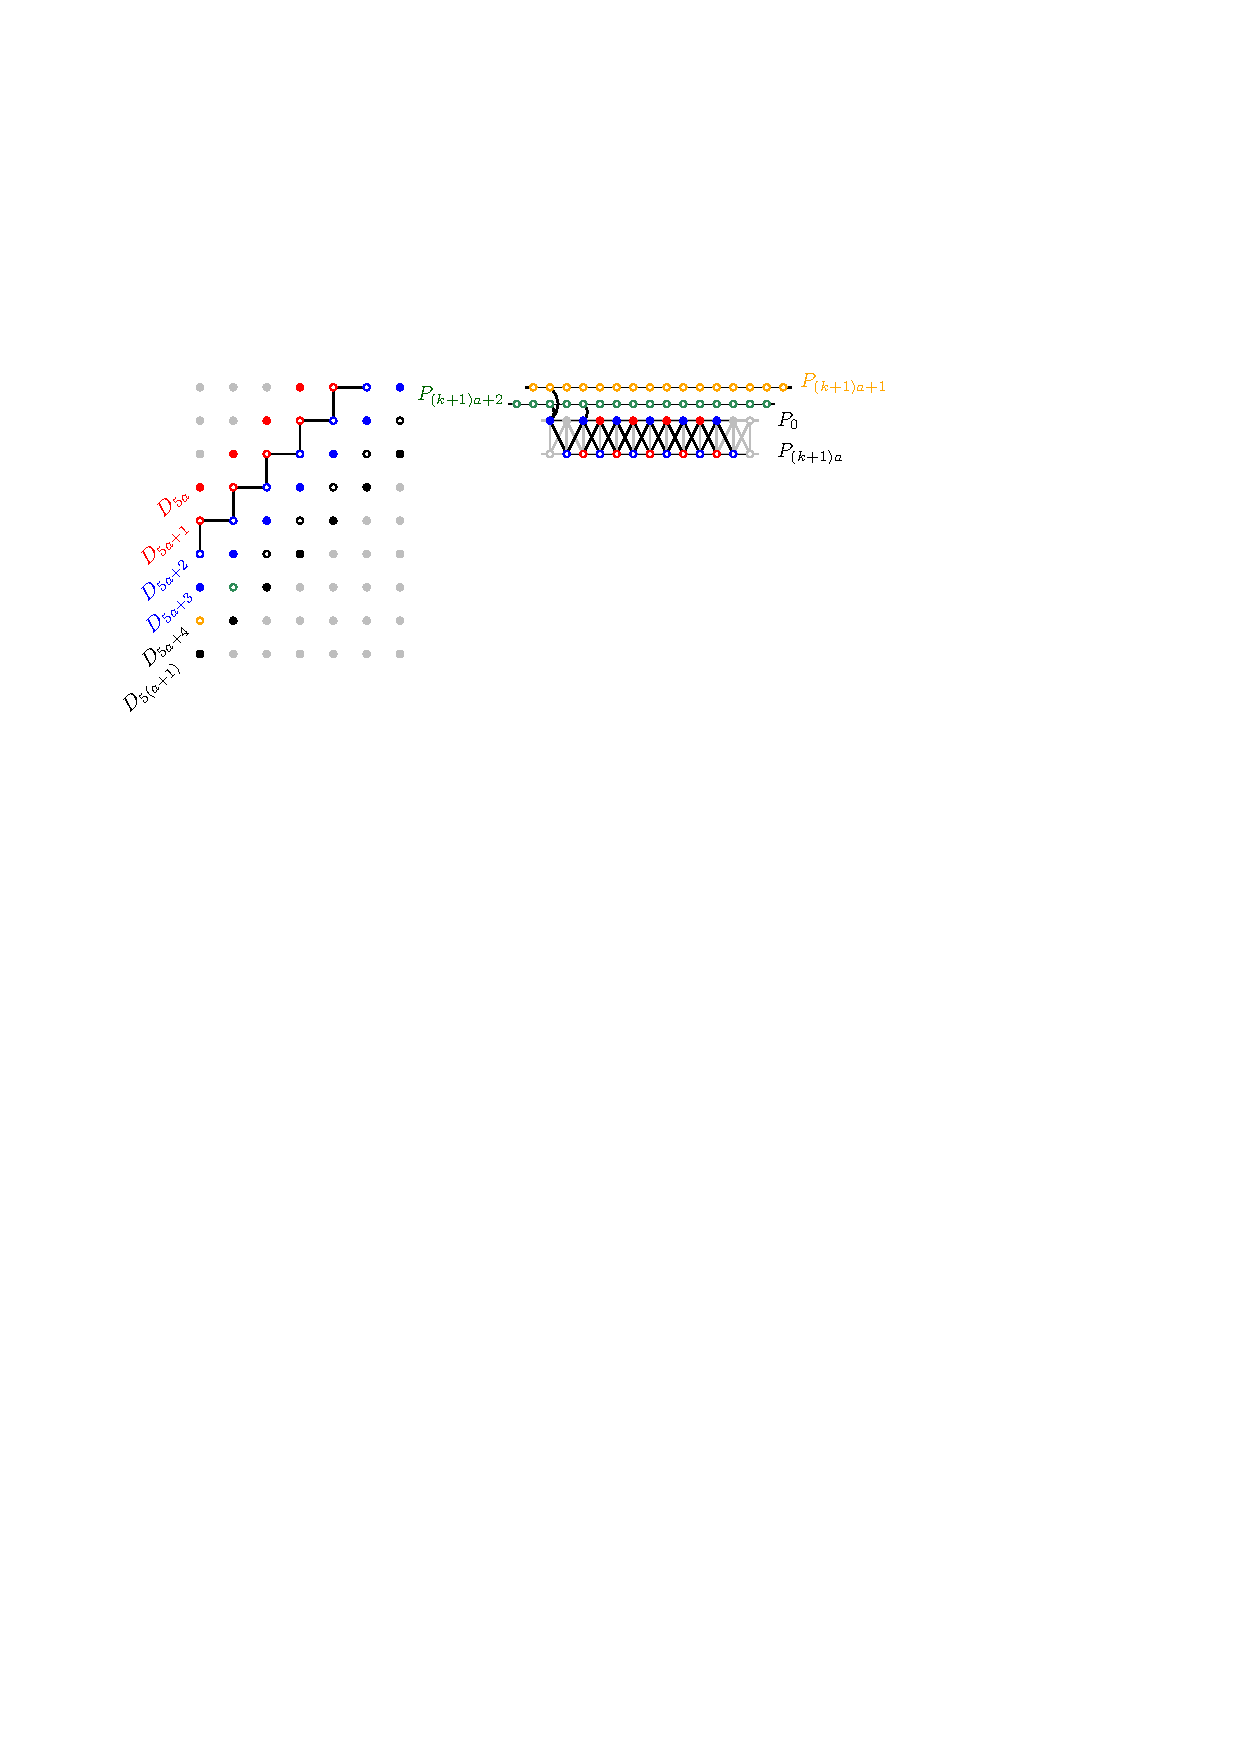
\includegraphics{figs/fivehalves.pdf}




\begin{lem}\label{star_times_tree_cartesian}
  For any star $S$ and any $n$-vertex tree $T$, 
  $$\gm(S\boxprod T)\le \sqrt{2n}+1.$$
\end{lem}

\begin{proof}
  Let $\mathcal{M}:=\{B_x:x\in V(\boxplus_k)\}$ be a model of $\boxplus_k$ in $G:=S\boxprod T$.  Let $v_0,\ldots,v_\mu$ denote the vertices of $S$, where $v_0$ has degree $\mu$ and $v_1,\ldots,v_\mu$ are leaves.  For each $i\in\{0,\ldots,\mu\}$ let $R_i:=\{v_i\}\boxprod V(T)$, so that $T_i:=G[R_i]$ is isomorphic to $T$.  The idea behind the rest of this proof is that the vertices in $R_0$ are special because each vertex in $R_0$ is adjacent to the corresponding vertex in each of $T_1,\ldots,T_\mu$. This makes the vertices in $R_0$ a scarce resource that the model $\mathcal{M}$ must use efficiently.  Let $X_0:=\{x\in V(\boxplus_k):B_x\cap R_0\neq\emptyset\}$ be the set of vertices in $\boxplus_k$ whose branch sets intersect $R_0$.

  Observe that $G-R_0$ is the vertex-disjoint union of trees $T_1,\ldots,T_\mu$.  Therefore, for each component $C$ of $\boxplus_k-X_0$, $G[\bigcup_{x\in V(C)} B_x]$ is a subtree of $T_i$ for some $i\in\{1,\ldots,\mu\}$.  Let $\mathcal{F}$ be the set of $4$-cycles in $\boxplus_k$. (So $\mathcal{F}$ is the set of inner faces in the usual plane drawing of $\boxplus_k$.)  Observe that, for each $F\in\mathcal{F}$, $|V(F)\cap X_0|\ge 1$ since otherwise $V(F)\subseteq X\setminus X_0$, so $\bigcup_{x\in V(F)}B_x\subseteq V(G-R_0)$ which implies that $F$ is a minor of $G-R_0$. This is not possible since $F$ is a cycle and $G-R_0$ is a forest.  
  
  Next we will show that $|\bigcup_{x\in V(F)} B_x\cap R_0|\ge 2$ for each $F\in\mathcal{F}$.  If $|V(F)\cap X_0|\ge 2$, then this is immediate, so suppose that $|V(F)\cap X_0|=1$.  Refer to \cref{star_times_tree_cartesian_fig}.  Let $F:=xx_1x_2x_3$ where $x\in X_0$ and $x_1,x_2,x_3\in X\setminus X_0$.  Since $G[\{x_1,x_2,x_3\}]$ is connected, there exists an $i\in\{1,\ldots,n\}$ such that $T'_j:=G[B_{x_j}]$ is a subtree of $T_i$ for each $j\in\{1,2,3\}$.  Furthermore, the subtree $T'_2$ is ``between'' $T'_1$ and $T'_3$ in the sense that $B_{x_1}$ and $B_{x_2}$ are in different components of $T_i-B_{x_2}$.  Since $N_{\boxplus_k}(x)$ contains both $x_1$ and $x_3$, $B_x$ contains vertices in $N_{G}(B_{x_1})$ and in  $N_{G}(B_{x_3})$.  Since $G[B_x]$ is connected, this implies that $G[B_x]$ contains a path from some vertex in  $N_{G}(B_{x_1})$ to some vertex in $N_{G}(B_{x_3})$.  Since $G[B_x]$ is a subgraph of $G-B_{x_2}$, this implies that any such path must contain at least two vertices of $R_0$.\footnote{This is true for the Cartesian product $S\boxprod T$, but not true for the strong product $S\boxtimes T$, since $N_{S\boxtimes T}(B_{x_1})$ and $N_{S\boxtimes T}(B_{x_3})$ can have a common vertex in $T_0$. This fact is used in the construction described in \cref{star_times_tree_strong}.}  Thus $|\bigcup_{x\in V(F)}B_x\cap R_0|=|B_x\cap R_0|\ge 2$, as claimed.

  \begin{figure}[ht]
    \centering
    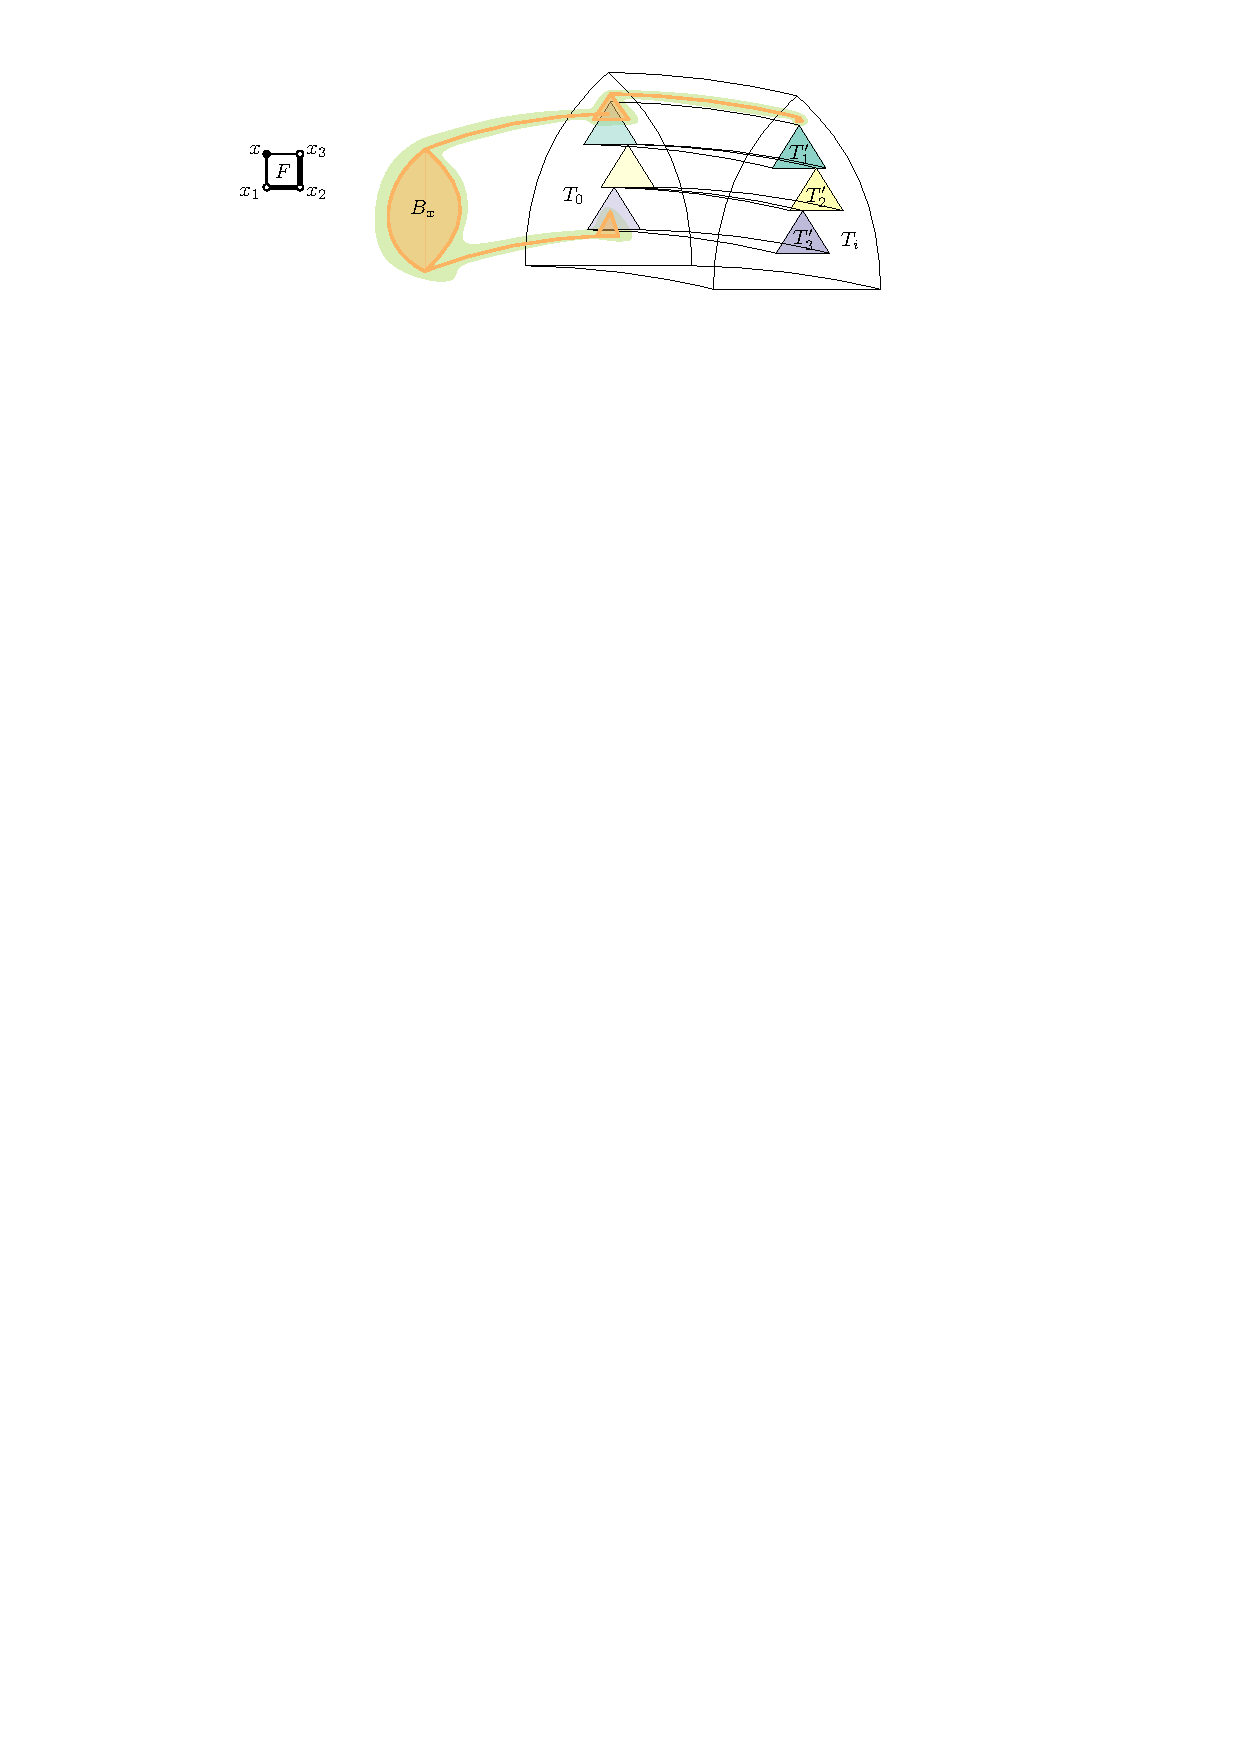
\includegraphics{figs/star_times_tree_cartesian}
    \caption{The proof of \cref{star_times_tree_cartesian}.}
    \label{star_times_tree_cartesian_fig}
  \end{figure}

  Now we can finish the proof with
  \[
    \sum_{F\in\mathcal{F}}\sum_{x\in V(F)} |B_x\cap R_0| \ge \sum_{F\in\mathcal{F}} 2 = 2|\mathcal{F}| = 2(k-1)^2 \enspace .
  \]
  Each vertex in $R_0$ appears in $B_x$ for at most one $x\in V(\boxplus_k)$, and each such $x$ appears in $V(F)$ for at most four cycles $F\in\mathcal{F}$, so 
  \[
    \sum_{F\in\mathcal{F}}\sum_{x\in V(F)} |B_x\cap R_0| \le 4\sum_{x\in V(\boxplus_k)} |B_x\cap R_0| \le 4|R_0| = 4n \enspace .
  \]
  Combining the previous two equations gives $4n\ge 2(k-1)^2$, so $k \le \sqrt{2n}+1$.
\end{proof}

\cref{uppercorr,star_times_tree_cartesian} together show that $c=2$ in \eqref{StarTreeQuestion}. 

Now consider \eqref{StarTreeQuestion} for the strong product $S\boxtimes T$. We now show that the answers for Cartesian and strong products are different. In particular, for $S\boxtimes T$ the minimum $c$ in \eqref{StarTreeQuestion} satisfies $\frac52 \leq c \leq 3$. 

\begin{lem}\label{star_times_tree_strong}
  For any star $S$ with at least $\sqrt{10(n-2)}+1$ leaves and any path $P$ on at least $n$ vertices, $$\gm(S\boxtimes P)\ge \lfloor\sqrt{5(n-2)/2}\rfloor$$
\end{lem}

\begin{proof}
  Let $k:=\lfloor\sqrt{5(n-2)/2}\rfloor$ and note that $n\ge 2k^2/5 + 2$.
  Let $G:=S\boxtimes P$. 
  Recall that $V(\boxplus_k)=\{1,\ldots,k\}^2$.  For each $i\in\{0,\ldots,2k-2\}$, let $D_i:=\{(x,y)\in V(\boxplus_k):y-x=k-i-1\}$,  and for convenience let $D_i=\emptyset$ for any $i\not\in\{0,\ldots,2k-2\}$. %\david{Not that it matters, but would it be cleaner to define $D_i:=\{(x,x-i)\in V(\boxplus_k):x\in[k]\}$ for $i\in\{1-k,\dots,k-1\}$? \pat{I tried, but then the indexing gets very confusing below.}} \david{okay}
  (The vertices of each $D_i$ are contained in a line of slope $1$.)  Let the vertices of $S$ be $v_0,\ldots,v_{2k+1}$, where $v_0$ is the vertex of degree $2k+1$ and  $v_1,\ldots,v_{2k+1}$ are the leaves.  
  % For each $i\in\{0,\ldots,2k+1\}$, let $P_i:=G[\{v_i\}\boxprod V(P)]$.

  For each $\ell\in\{0,\ldots,4\}$, let $\alpha_\ell:=|\bigcup_{a\in\mathbb{Z}} D_{\ell+5a+1}\cup D_{\ell+5a+2}|$.  Observe that $\sum_{\ell=0}^4 \alpha_\ell=2|V(\boxplus_k)|=2k^2$, since each diagonal $D_i$ contributes to this sum exactly twice (when $i-\ell\equiv 1\pmod 5$ and when $i-\ell\equiv 2\pmod 5$).  Therefore, $\alpha_\ell\le 2k^2/5$ for some $\ell\in\{0,\ldots,4\}$.  For the sake of brevity, assume that $\alpha_0\le 2k^2/5$.  (The only reason for this assumption is to avoid having to include an $\ell$ term in many of the subscripts in the following paragraphs.)
  
  % Let the vertices of $P$ be $w_1,\ldots,w_n$, in the order they appear along $P$.  

  We now explain how to embed a small (width-$4$) strip $B_a$ of $\boxplus_k$ into a small subgraph $S\subseteq G[\{v_0,v_1\}\times V(P)]$ of $G$.  This will allow us to decompose $\boxplus_k$ into disjoint independent strips and embed them all on $G[\{v_0,v_1\}\times V(P)]$.  We will then complete the embedding by embedding the remaining (width-$1$) strips into $G[\{v_2,\ldots,v_{k+1}\}\times V(P)\}]$.  Fix some integer $a\in\{0,\ldots,\lfloor 2k/5\rfloor-1\}$, and consider the induced subgraph $B_a:=\boxplus_k[D_{5a}\cup\cdots \cup D_{5a+3}]$.  Let $S':=S[\{v_0,v_1\}]$ and let $P_a'$ be any  subpath of $P$ with $|D_{5a+1}\cup D_{5a+2}|$ vertices.  As illustrated in \cref{fivehalves}, $G':=S'\boxtimes P_a'$ contains a subgraph isomorphic to $B_a$, where the isomorphism $\varphi:B_a\to G'$ maps the vertices of $D_{5a}\cup D_{5a+3}$ onto the vertices in $\{v_0\}\times V(P_a')$.  (Note that this makes use of the fact that $|D_{5a}\cup D_{5a+3}|\le |D_{5a+2}\cup D_{5a+2}|$, valid for all $a\in\{0,\ldots,2k-5\}$.  Since $P_a'$ uses only $|D_{5a+1}\cup D_{5a+2}|$ vertices of $P$, this immediately implies that $G[\{v_0,v_1\}\times V(P)]$ contains a subgraph isomorphic to $X:=\boxplus_k-\bigcup_{a\ge 0}D_{5a+4}$.\footnote{Recall that $P$ has $n\ge 2k^2/5+2\ge \alpha_0+2$ vertices. The additional two vertices are required for two boundary cases where we can only guarantee that $|D_{\ell+5a+1}\cup D_{\ell+5a+2}|+1\ge |D_{\ell+5a}\cup D_{\ell+5a+3}|$.  These cases can occur when $\ell+5a=-2$ (because $|D_{-1}\cup D_0|=1$ and $|D_{-2}\cup D_{1}|=2$ and when $\ell+5a=2k-3$ (because $|D_{2k-2}\cup D_{2k-1}=1$ and $|D_{2k-3}\cup D_{2k}|=2$).} Furthermore, the vertex disjoint subpaths $P'_a$, $a\in \mathbb{Z}$ can be chosen so that $P'_a$ and $P'_{a+1}$ are always consecutive in $P$.
  
  \begin{figure}[ht]
    \centering
    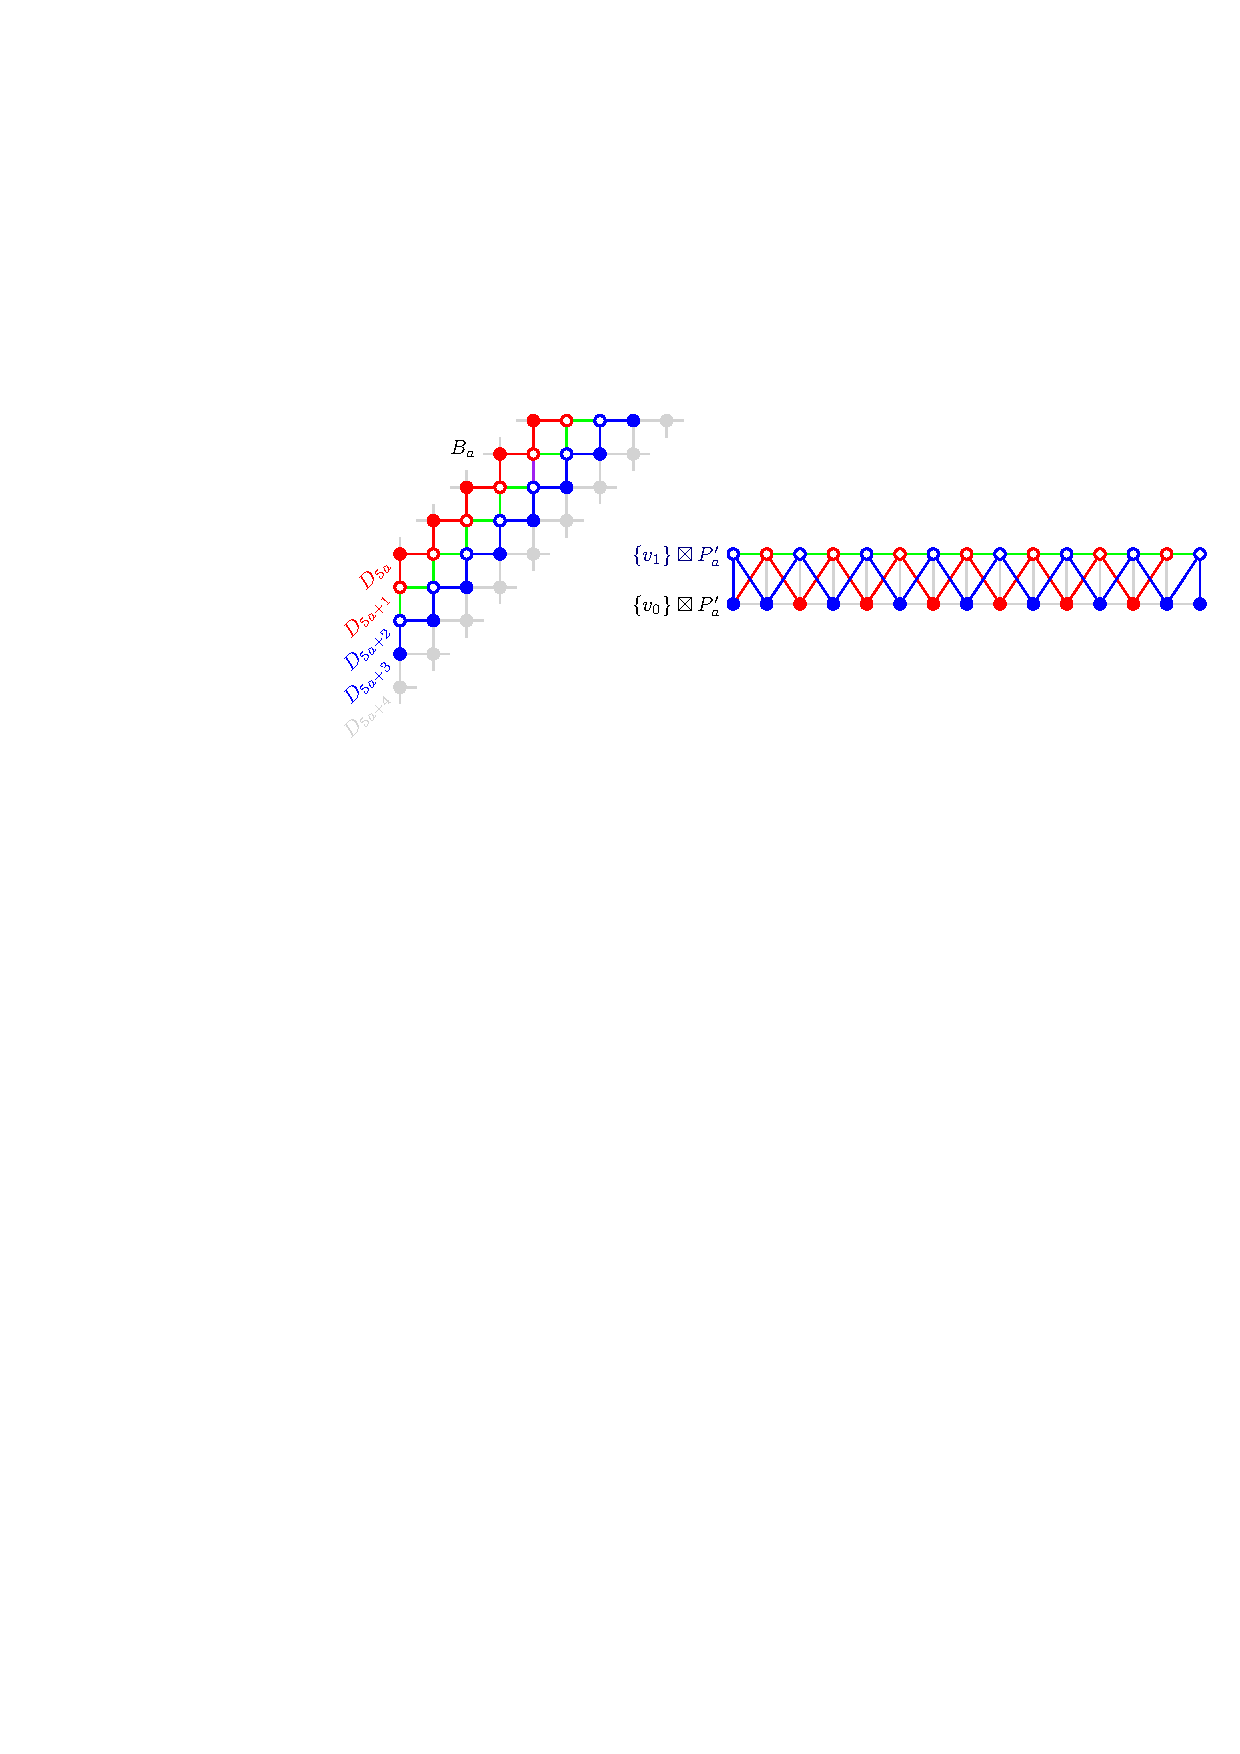
\includegraphics{figs/fh2.pdf}
    \caption{The construction in \cref{star_times_tree_strong}. }
    \label{fivehalves}
  \end{figure}

  By setting $B_x:=\{\varphi(x)\}$ for each $x\in V(X)$ we immediately obtain a model $\{B_x:x\in V(X)\}$ of $X$ in $G$.  We can complete this model of $X$ to a model of $\boxplus_k$ by mapping, for each $a\equiv 4\pmod 5$, the at most $k$ vertices in $D_{5a+4}$ to subsets of $\{v_2,\ldots,v_{2k+1}\}\times P$.  More precisely, let $x_1,\ldots,x_r$ be the vertices in $D_{5a+4}$.  These vertices have neighbours in $D_{5a+3}$ and in $D_{5(a+1)}$.  The vertices in $D_{5a+3}$ have branch sets in $\{v_0\}\times V(P'_a)$.  The vertices in $D_{5(a+1)}$ have branch sets in $\{v_0\}\times V(P'_{a+1})$.  If $a$ is even then we set $B_{x_i}:=\{v_{2i}\}\times (V(P'_a)\cup V(P'_{a+1}))$.  If $a$ is odd then we set $B_{x_i}:=\{v_{2i+1}\}\times (V(P'_a)\cup V(P'_{a+1}))$.  This ensures that $B_{x_i}$ is adjacent to the branch sets of $x_i$'s neighbours in $D_{5a+3}$ and $D_{5(a+1)}$.  Using different subsets of $v_2,\ldots,v_{2k+1}$ for odd and even values of $a$ ensures that the branch sets of vertices in $D_{5a+4}$ are disjoint from those of vertices in $D_{5(a+1)+4}$.  This completes the proof.
\end{proof}
  

% \worley{would the rootless vertices in $D_3$ at the end of the diagonals only be adjacent to one rooty vertex, the adjacent one from $D_2$?}

% \worley{The diagonals WWgive $10\floor{k/5}^2 + 4\floor{k/5}$ rooty vertices}

To complete this section, we now show that for lexicographic products $S\cdot T$, the answer to \eqref{StarTreeQuestion} is $c=3$. By \cref{StarTreeUpperBound}, it suffices to prove the following (where $P_3=S_2$ is the star with two leaves):

% \begin{prop}
% \label{LexST}
% For any integer $n\geq 12$, for any star $S$ with at least $\sqrt{4n/3}$ leaves, and for any path on at least $n$ vertices, 
% $$\gm(S\cdot P)\geq \floor{\sqrt{3n}}.$$
% \end{prop}

% \begin{proof}
% Let $k:=\floor{\sqrt{3n}}$. We in fact show that $\boxplus_{k}$ is isomorphic to a subgraph of $S\cdot P$. Recall that $\boxplus_{k}$ has vertex-set $[k]^2$. For each $i\in\mathbb{Z}$, let $D_i:=\{(x,x+i):x,x+i\in[k]\}$. Each $D_i$ is an independent set in $\boxplus_{k}$ contained in a diagonal line of slope $1$, and $D_i\neq\emptyset$ if and only if $i\in[1-k,k-1]$. For $j\in\{0,1,2\}$, let $X_j:=\bigcup\{D_{3i}+j:i\in\mathbb{Z}\}$. So $X_0,X_1,X_2$ partitions $V(\boxplus_k)$, and each $X_j$ is an independent set in $\boxplus_k$. For some $j\in\{0,1,2\}$, we have $|X_j|\leq k^2/3$. Let $I:=\{i\in\mathbb{Z}: 1-k\leq 3i+j+1\text{ and }3i+j+2\leq k-1\}$. By assumption, the number of leaves in $S$ is at least $\sqrt{4n/3}\geq \frac23 k \geq |I|$ leaves. Let $(v_i:i\in I)$ be distinct leaves in $S$. Let $r$ be the non-leaf vertex in $S$. For each $i\in I$, let $P_i:=\boxplus_{k}[D_{3i+j+1}\cup D_{3i+j+2}]$ which is a path in $\boxplus_{k}$ on at most $2k$ vertices, as illustrated in \cref{LexSTfig}. Note that $(P_i:i\in I)$ partitions $V(\boxplus_{k})\setminus X_j$, and there is no edge between $P_i$ and $P_{i'}$ for distinct $i,i'\in[??]$. Injectively map $X_j$ to the path $\{r\}\cdot V(P)$ in $S\cdot P$, which is possible since $|X_j|\leq k^2/3\leq n\leq |V(P)|$. For each $i\in I$, injectively and homomorphically map $P_i$ to the path $\{v_i\}\cdot V(P)$ in $S\cdot P$, which is possible since $|V(P)|=n\geq k^2/3\geq 2k\geq |V(P_i)|$. This defines an injection from $V(G)$ to $V(S\cdot P)$. Observe that each edge of $\boxplus_k$ is mapped to an edge of $S\cdot P$. Hence $G$ is isomorphic to a subgraph of $S\cdot P$, as desired. 
% \end{proof}

\begin{lem}
$\boxplus_k$ is isomorphic to a subgraph of $P_3 \cdot P_n$, where $k=\floor{\sqrt{3n-2}}$.
\label{LexST}
\end{lem}

\begin{proof}
Recall that $\boxplus_{k}$ has vertex-set $[k]^2$. 
For each $i\in\mathbb{Z}$, let $D_i:=\{(x,x+i):x,x+i\in[k]\}$. Each $D_i$ is an independent set in $\boxplus_{k}$ contained in a diagonal line of slope $1$. 
As illustrated in \cref{LexSTfig}, 
let $S:=\bigcup\{D_{i}:i\equiv 0\pmod{3}\}$, 
which is an independent set in $\boxplus_k$. 
Let $A:=\bigcup\{D_{i}:i\not\equiv 0\pmod{3}, i>0\}$ and
 $B:=\bigcup\{D_{i}:i\not\equiv 0\pmod{3}, i<0\}$. 
Each of $A$ and $B$ induce linear forests in $\boxplus_k$.  
Note that $S,A,B$ partitions $V(\boxplus_k)$, and $\floor{k^2/3}\leq|S|,|A|,|B|\leq\ceil{k^2/3}\leq n$. 
Consider the 3-vertex path $P_3=(a,s,b)$. 
Injectively map $S$ to the the copy of $P_n$ corresponding to $s$. Injectively and homomorphically map $A$ to the copy of $P_n$ corresponding to $a$. Similarly, injectively and homomorphically map $B$ to the copy of $P_n$ corresponding to $b$. This defines an injection from $V(\boxplus_k)$ to $V(P_3\cdot P_n)$. Since there is no edge of $\boxplus_k$ between $A$ and $B$, each edge of $\boxplus_k$ is mapped to an edge of $P_3\cdot P_n$, and $\boxplus_k$ is isomorphic to a subgraph of $P_3\cdot P_n$.
\end{proof}


\begin{figure}[ht]
\centering
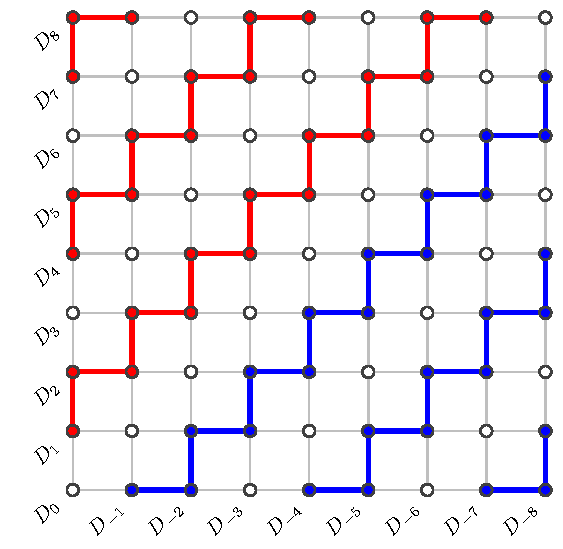
\includegraphics[scale=0.7]{figs/LexST.pdf}
\caption{The proof of \cref{LexST} with $k=9$: vertices in $S$ are white, red paths are in $A$, and blue paths are in $B$.}
\label{LexSTfig}
\end{figure}


\section{Open Problems}\label{E}

%\pat{I suggest we remove the following paragraph:} \david{I agree.}  \cref{quadratic_grid_minor} shows the existence of very simple graph products that do not have the linear (or even subquadratic) grid minor property.  Thus, the SQGM Framework for optimization problems on graphs with the subquadratic grid minor property does not immediately apply \david{The SQGM Framework needs to be explained before we say it does not apply.}.  Nevertheless, these graph products are still highly structured, so there may be a general framework for attacking these types of problems on (subgraphs of) graph products.  If so, this will require new ideas: The prototypical problem for the SQGM Framework is \textsc{FeedbackVertexSet} which asks for the smallest $S\subseteq V(G)$ such that $G-S$ is a forest. A critical property of the SQGM framework is that the size of an optimal solution for a graph of treewidth $k$ should be $\Omega(k^{1+\delta})$ for some $\delta>0$.  Unfortunately, $S_n\boxprod P_n$ has treewidth $2n-1$ (or so) but has a feedback vertex set of size $n$ (every copy of the root of $S_n$).

An open problem is to tighten the bounds for $\gm(S\boxtimes T)$ presented in \cref{StarTreeUpperBound} and \cref{star_times_tree_strong}, which combine to show that $\sqrt{5(n-2)/2} \le \gm(S\boxtimes T) \le \sqrt{3n+1}+1$.
This would fully resolve the discussions resulting from \eqref{StarTreeQuestion}.

Another area of future work is to further investigate the implications of the Planar Graph Product Structure Theorem, which we recall states that for every planar graph $G$, there exists a graph $H$ of bounded treewidth and a path $P$ such that $G \subsetsim H \boxtimes P$. A specific area to investigate is identifying which properties of the planar graph $G$ can be preserved in the strong product $H\boxtimes P$ that contains $G$~\cite{DJMMUW20}.   Several results of this type are known. For example, in the proof of \citet{DJMMUW20}, $H$ is a minor of $G$, and so $H$ is planar. An impossibility result in this area is the following: Even if $G$ is planar and has maximum-degree $5$, a result of the form $G\subseteq H\boxtimes P$ cannot guarantee that $H$ has bounded treewidth and bounded degree~\cite{DJMMW22}.  

A concrete question that remains open is whether the treewidth of $G$ can be preserved in the product:
Is it true that for every planar graph $G$, there exists a bounded treewidth graph $H$ and a path $P$ such that $G\subsetsim H\boxtimes P$ and $\tw(H\boxtimes P) \in O(\tw(G))$? Note that 
$$\Omega(\min\{|V(H)|,|V(P)|\})\leq  \tw( H\boxtimes P) \leq O(\min\{|V(H)|,|V(P)|\}).$$ 
This upper bound holds since $\tw(G_1\boxtimes G_2)\leq (\tw(G_1)+1)|V(G_2)|-1$ for all graphs $G_1,G_2$, and both $H$ and $P$ have bounded treewidth. The lower bound follows from \eqref{LowerBoundProduct} since we may assume that $G$, $H$ and $P$ are connected. So this question really asks whether for every planar graph $G$, there exists a bounded treewidth graph $H$ and a path $P$ such that $G\subsetsim H\boxtimes P$ and $\min\{|V(H)|,|V(P)|\} \leq O(\tw(G))$. It is even open whether $\min\{|V(H)|,|V(P)|\} \leq f(\tw(G))$ for some function $f$, or whether $\min\{|V(H)|,|V(P)|\} \leq O(\sqrt{|V(G)|})$ (which would be implied since $\tw(G) \leq O(\sqrt{|V(G)|})$ for every planar graph $G$).

{\fontsize{10pt}{11pt}\selectfont
\bibliographystyle{DavidNatbibStyle}
\bibliography{DavidBibliography,additionalbiblio}}
\end{document}

